\section{Analysis method}
\label{sec:method}

This section documents the thrust analysis method, including the observable
definition, the response construction, the unfolding setup, systematic execution,
and the correction and covariance workflow. Executable workflow details, command
sequences, and pseudocode are collected in
Appendix~\ref{sec:app_workflow_code} to keep the main text focused on physics.

\subsection{Observable definition and nominal configuration}

The thrust observable is defined as~\cite{PhysRevLett.39.1587}
\begin{equation}
T = \max_{\hat{n}} \frac{\sum_i |\vec{p}_i \cdot \hat{n}|}{\sum_i |\vec{p}_i|},
\end{equation}
with all selected charged and neutral reconstructed objects from Sec.~\ref{sec:event_selection} entering the sum.
We first adopt bins identical to the published ALEPH event-shape analysis~\cite{Heister:2003aj}, using 50 uniform bins over $0.5 \le T < 1.0$ (bin width $\Delta T = 0.01$), which enables a direct bin-by-bin comparison with the published ALEPH result. We then test fine bins throughout the full thrust space to assess the usable binning resolution in different regions, particularly in the high-thrust (low $\tau = 1-T$) regime. The thrust resolution study in Sec.~\ref{sec:thrust_resolution} informs the finest binning achievable in each region.

\begin{table}[t!]
\centering
\begin{tabularx}{0.98\textwidth}{p{0.33\textwidth} X}
\hline
Item & Nominal configuration \\
\hline
Observable & Thrust $T$ \\
Range & $0.5 \le T < 1.0$ \\
Binning & 50 uniform bins \\
Reco/gen matching key & \texttt{uniqueID} \\
Reco selection branch & \texttt{passEventSelection} \\
Nominal IBU iterations & 5 \\
Hadronic correction & enabled ($N_{\mathrm{genBefore}}/N_{\mathrm{gen}}$) \\
Statistical covariance input & unfolding covariance transformed to normalized differential-thrust basis \\
RooUnfold covariance method & \texttt{kCovariance} (analytical error propagation) \\
Particle-level target & stable hadrons ($c\tau > 10$~mm), inclusive over full hadronic Z phase space \\
\hline
\end{tabularx}
\caption{Nominal analysis configuration used in the thrust Iterative Bayesian Unfolding workflow.}
\label{tab:method_config}
\end{table}


The nominal run uses $N_{\mathrm{iter}}=5$ and applies the post-unfolding hadronic event correction from
\texttt{tgenBefore/tgen}.
The nominal branch is the only run with covariance enabled; variation branches are propagated through signed shifts relative to the nominal spectrum.

\subsection{Response construction from matched MC}

Response filling uses event-by-event matching through \texttt{uniqueID}. Reconstructed MC entries with
\texttt{passEventSelection} equal to 1 define the selected detector-level phase space. Generator-level entries are then matched to this selected set and used to fill:
\begin{itemize}
\item the response counts matrix;
\item the miss term required by RooUnfold for inefficiency handling.
\end{itemize}

This matched-response construction enforces a consistent phase-space definition between detector-level selection and generator-level truth used in unfolding. Generator-level events with no matched reco entry (misses, from reconstruction inefficiency or acceptance gaps) are handled by RooUnfold's efficiency correction. Reco-level events with no matched gen entry (fakes, from beam background or random coincidences) are not expected to be significant in the archived ALEPH hadronic sample and are not separately subtracted.

\subsection{Iterative Bayesian Unfolding setup and iteration choice}

Detector correction is performed with RooUnfold Bayesian unfolding,
\begin{equation}
U_j^{(n+1)} = \frac{1}{\epsilon_j}\sum_i M_i\,\frac{R_{ij}\,\pi_j^{(n)}}{\sum_k R_{ik}\,\pi_k^{(n)}},
\end{equation}
where $M_i$ is the measured detector-level spectrum, $R_{ij}$ is the response, and $\pi_j^{(n)}$ is the iteration prior.

The prior for the first iteration is taken as the generator-level MC truth distribution $\pi_j^{(0)} = N_{\mathrm{gen}}(j)$, the standard RooUnfold default. This choice initializes the unfolding close to the expected truth shape and avoids any flat-prior amplification of high-frequency fluctuations in the first iteration.

The nominal regularization is
\begin{equation}
N_{\mathrm{iter}}=5,
\end{equation}
with $N_{\mathrm{iter}}=4$ and $6$ propagated as unfolding-regularization systematic branches.
The iteration-choice diagnostics are shown in
Figs.~\ref{fig:refold_selected_iters} and~\ref{fig:iteration_choice_diagnostics}, including $N=4,5,6,10,100$ refolding checks.

The response matrix has a diagonal fraction of $f_{\mathrm{diag}}=0.33$, meaning approximately two-thirds of events migrate out of their generated thrust bin at reconstruction level. This level of bin-to-bin migration is expected for thrust at ALEPH given the finite charged-particle momentum resolution and the sensitivity of thrust to soft particles near the event boundary. It implies that the unfolding correction is non-trivial and that the choice of regularization strength meaningfully affects the result. The iteration diagnostics in Fig.~\ref{fig:iteration_choice_diagnostics} show that the closure-shape $\chi^2/\mathrm{ndf}$ is stable and the iteration-to-iteration change in the unfolded spectrum is small for $N_{\mathrm{iter}} \in \{4,5,6\}$, providing confidence that $N_{\mathrm{iter}}=5$ sits in a well-regularized plateau rather than near an instability. The propagated $N_{\mathrm{iter}}=4,6$ systematic covers residual regularization-bias uncertainty at the level documented in Sec.~\ref{sec:systematics}.

The ``miss'' term---generator-level events with no matched reconstructed counterpart---is
documented in Fig.~\ref{fig:miss_term_efficiency}. These are events that fail the
reco-level hadronic event selection despite being generated within the fiducial volume.
The miss rate is concentrated at low thrust ($T\lesssim0.7$) and in events with low
charged multiplicity, consistent with the hadronic event selection removing poorly
reconstructed events. RooUnfold accounts for miss events via
\texttt{response.Miss($x_{\mathrm{gen}}$)}, which correct the unfolded spectrum for
this acceptance effect.

\begin{figure}[t!]
\centering
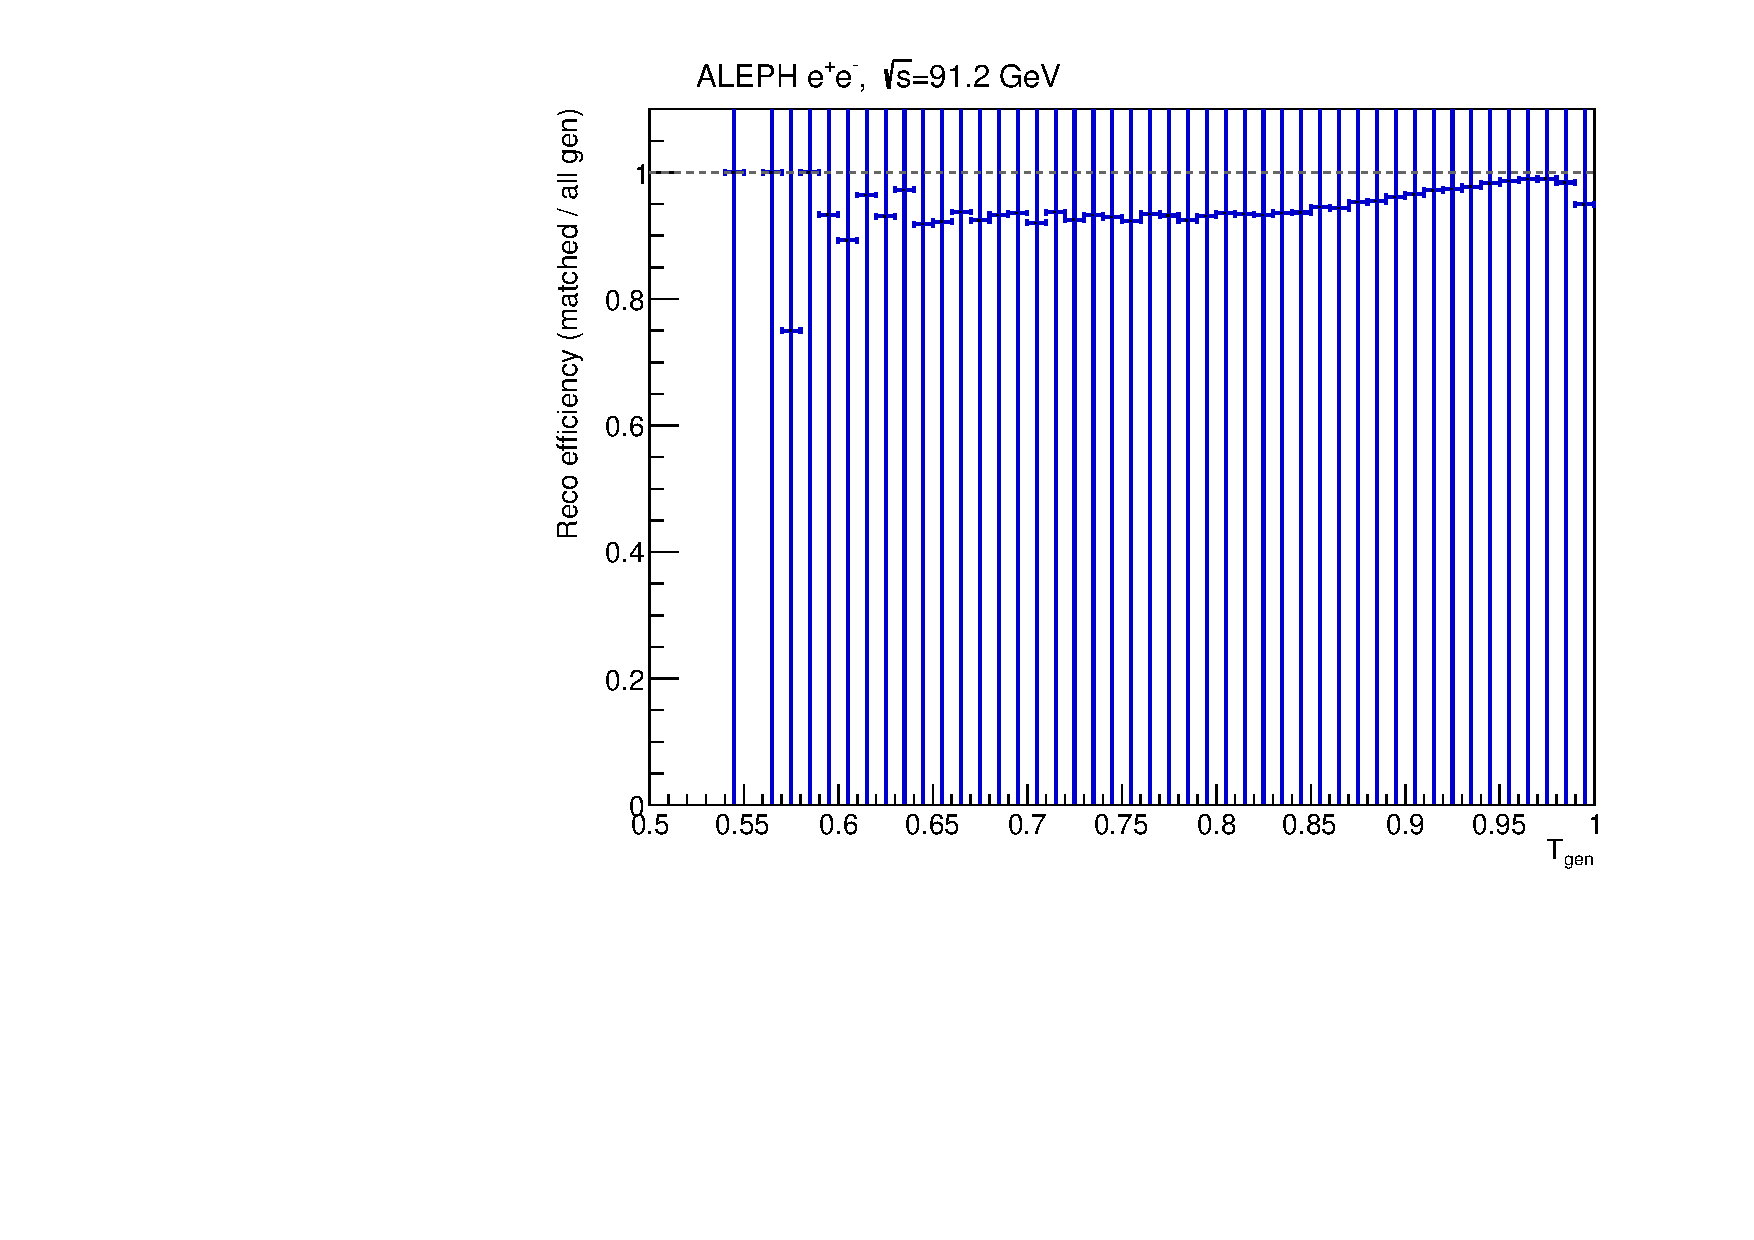
\includegraphics[width=0.49\textwidth]{../Studies/Phase2_Checks_2026-03-03/plots/miss_term/miss_term_efficiency.pdf}
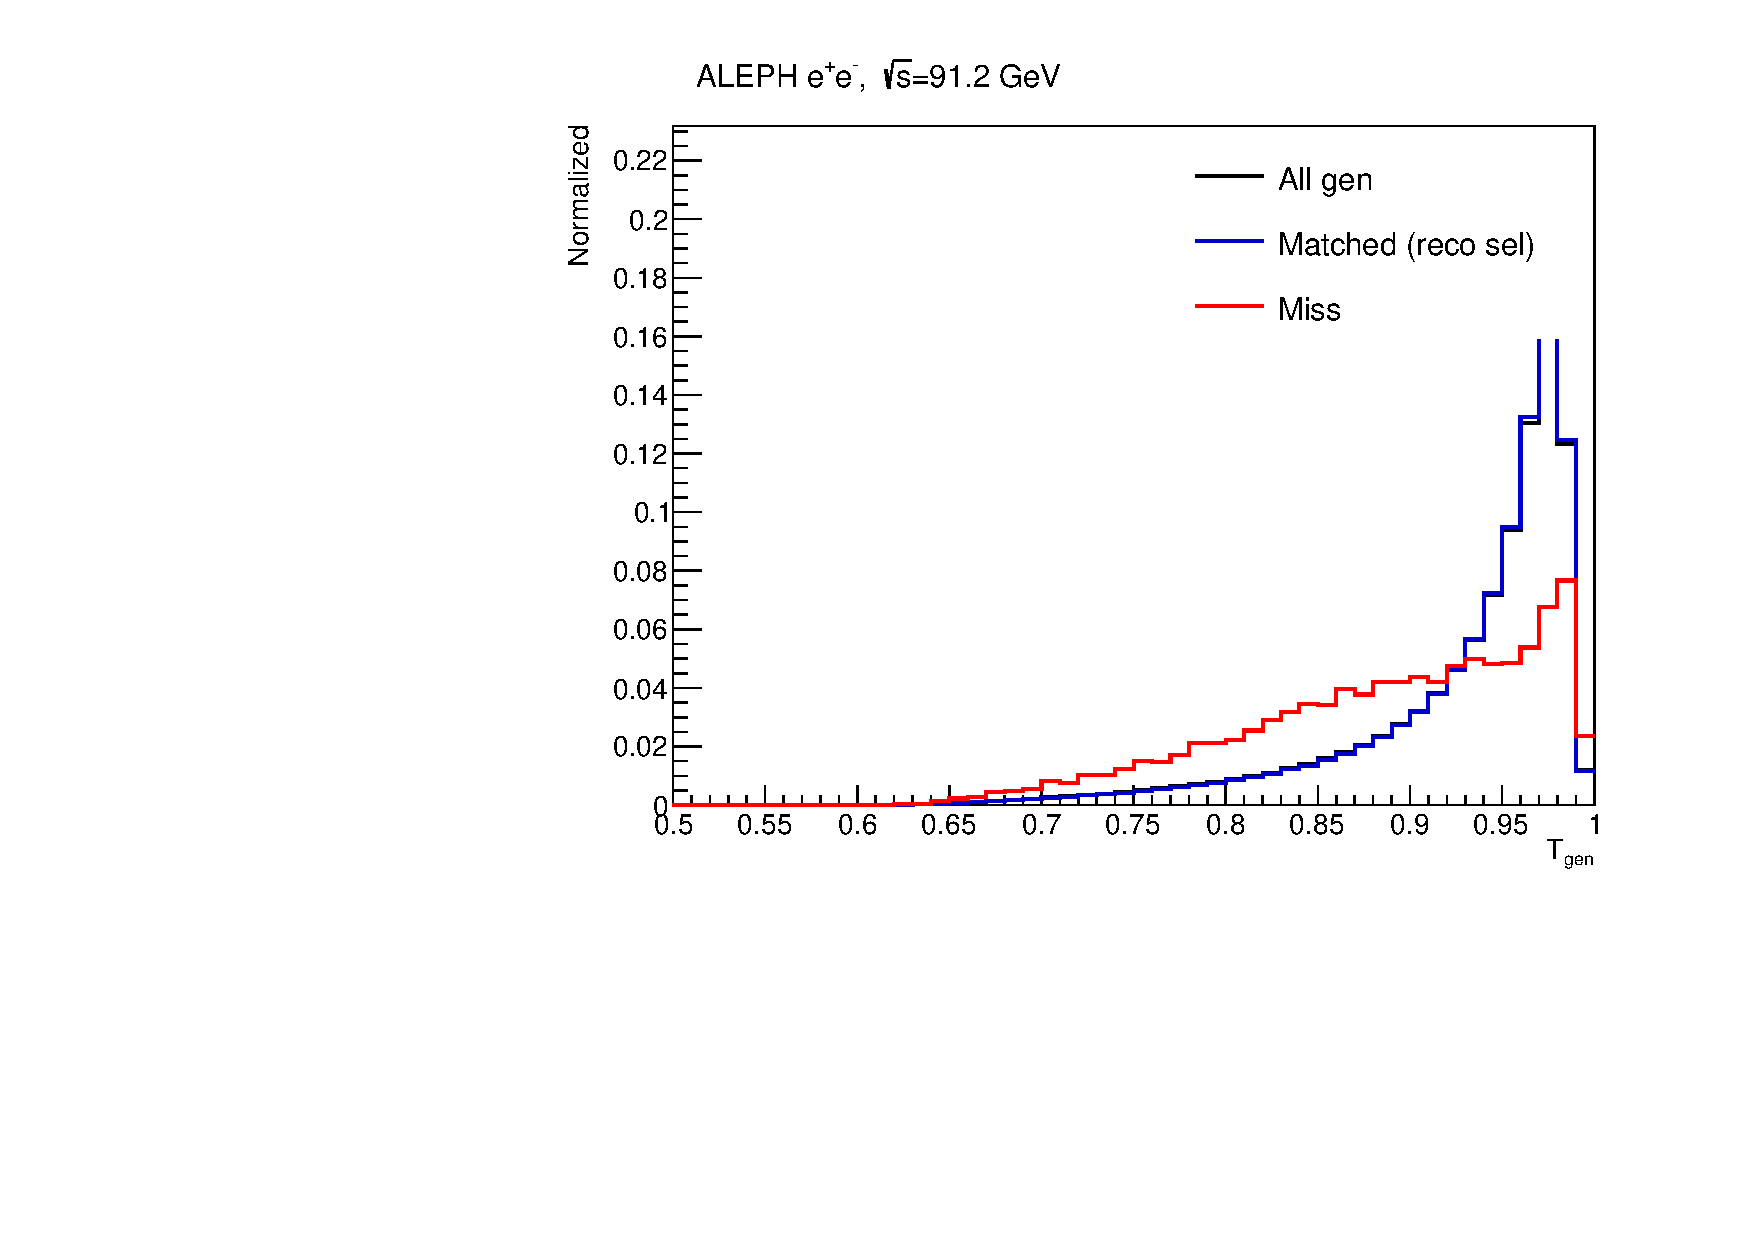
\includegraphics[width=0.49\textwidth]{../Studies/Phase2_Checks_2026-03-03/plots/miss_term/miss_term_thrust.pdf}
\caption{Left: reco efficiency (matched/all gen) as a function of $T_{\mathrm{gen}}$.
Right: thrust distributions for all gen, matched, and miss events (normalized to unit area).
Miss events are concentrated at low thrust and low multiplicity, consistent with
events failing the hadronic event selection.}
\label{fig:miss_term_efficiency}
\end{figure}

\begin{figure}[t!]
\centering
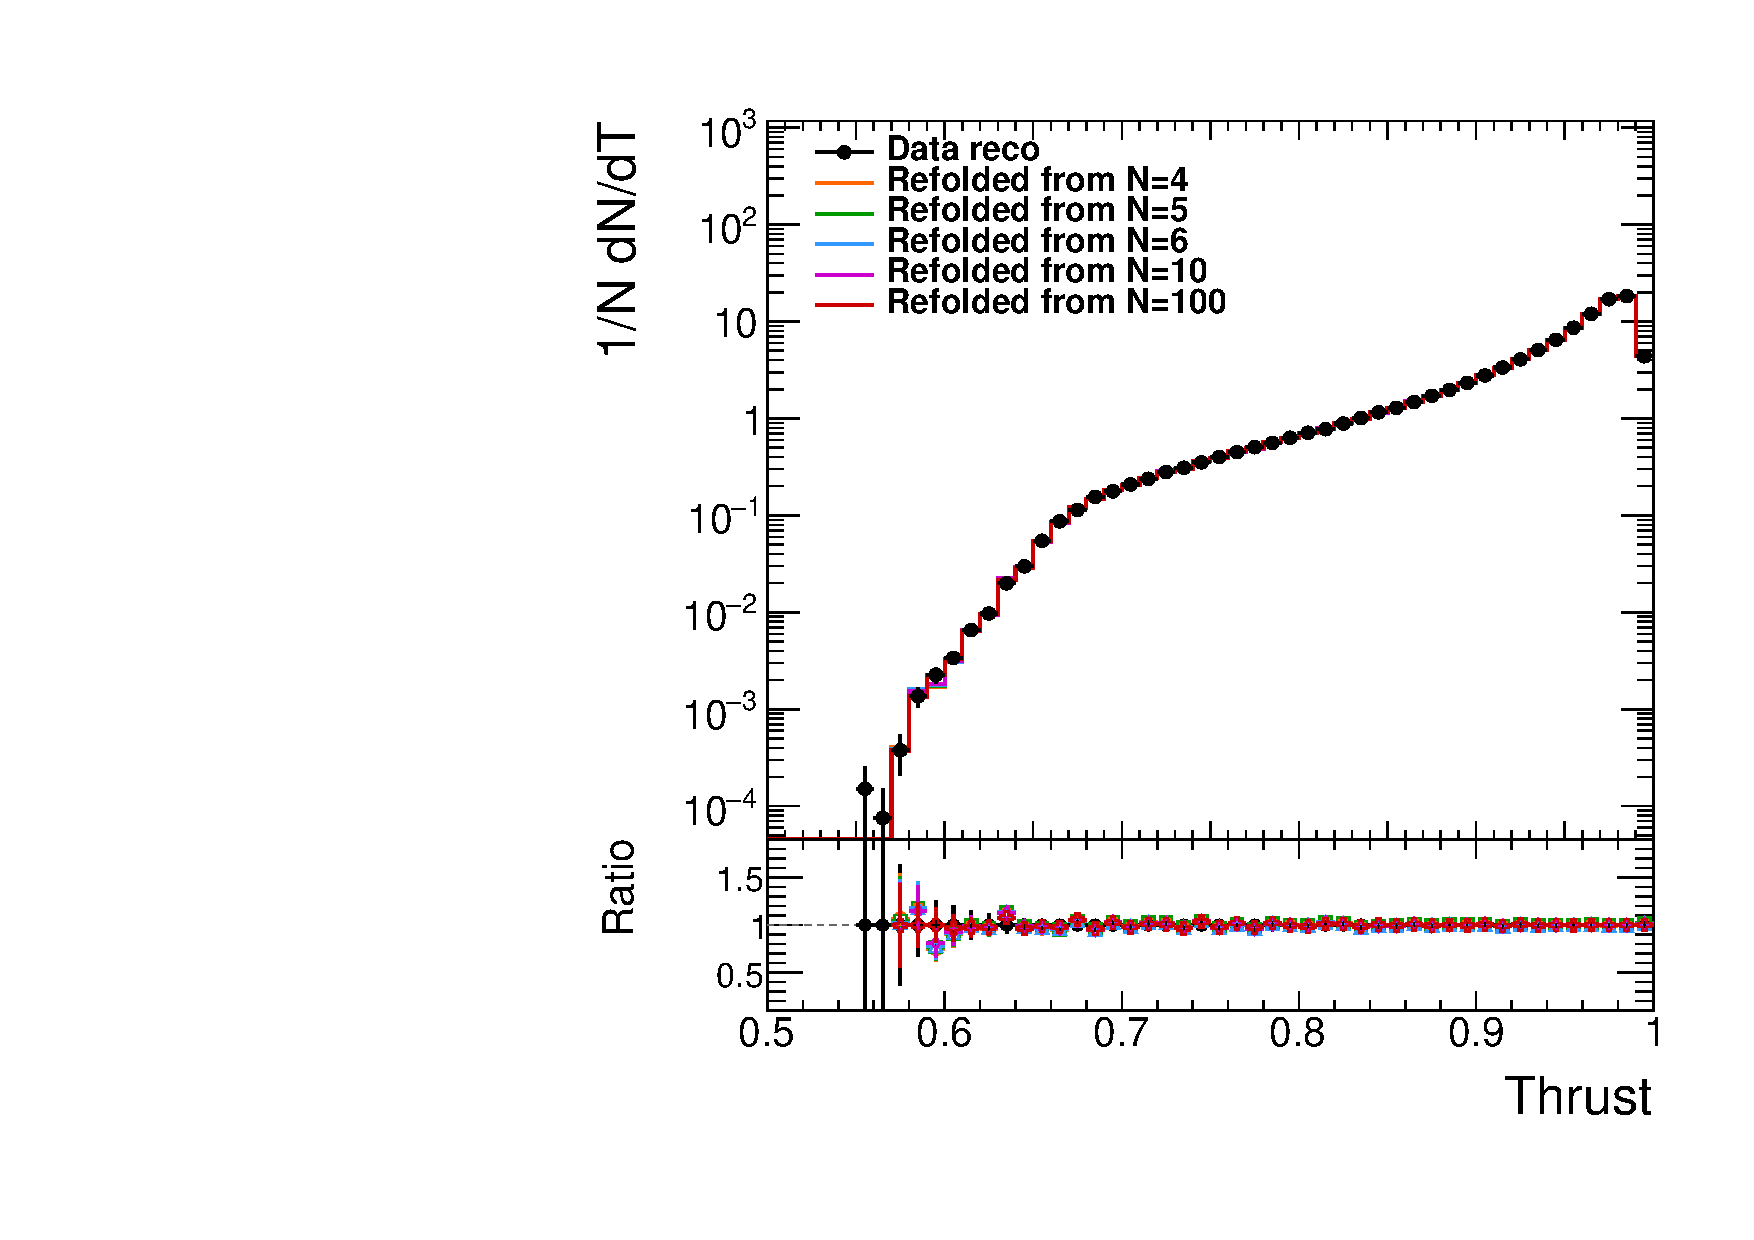
\includegraphics[width=0.65\textwidth]{../Studies/PreliminaryResult/2026-02-17_thrust_iter5/validation/iteration_scan/dist_refolded_vs_data_selected_iterations.pdf}
\caption{Refolded spectra from selected iteration points ($N_{\mathrm{iter}}=4,5,6,10,100$) compared with detector-level data.}
\label{fig:refold_selected_iters}
\end{figure}

\begin{figure}[t!]
\centering
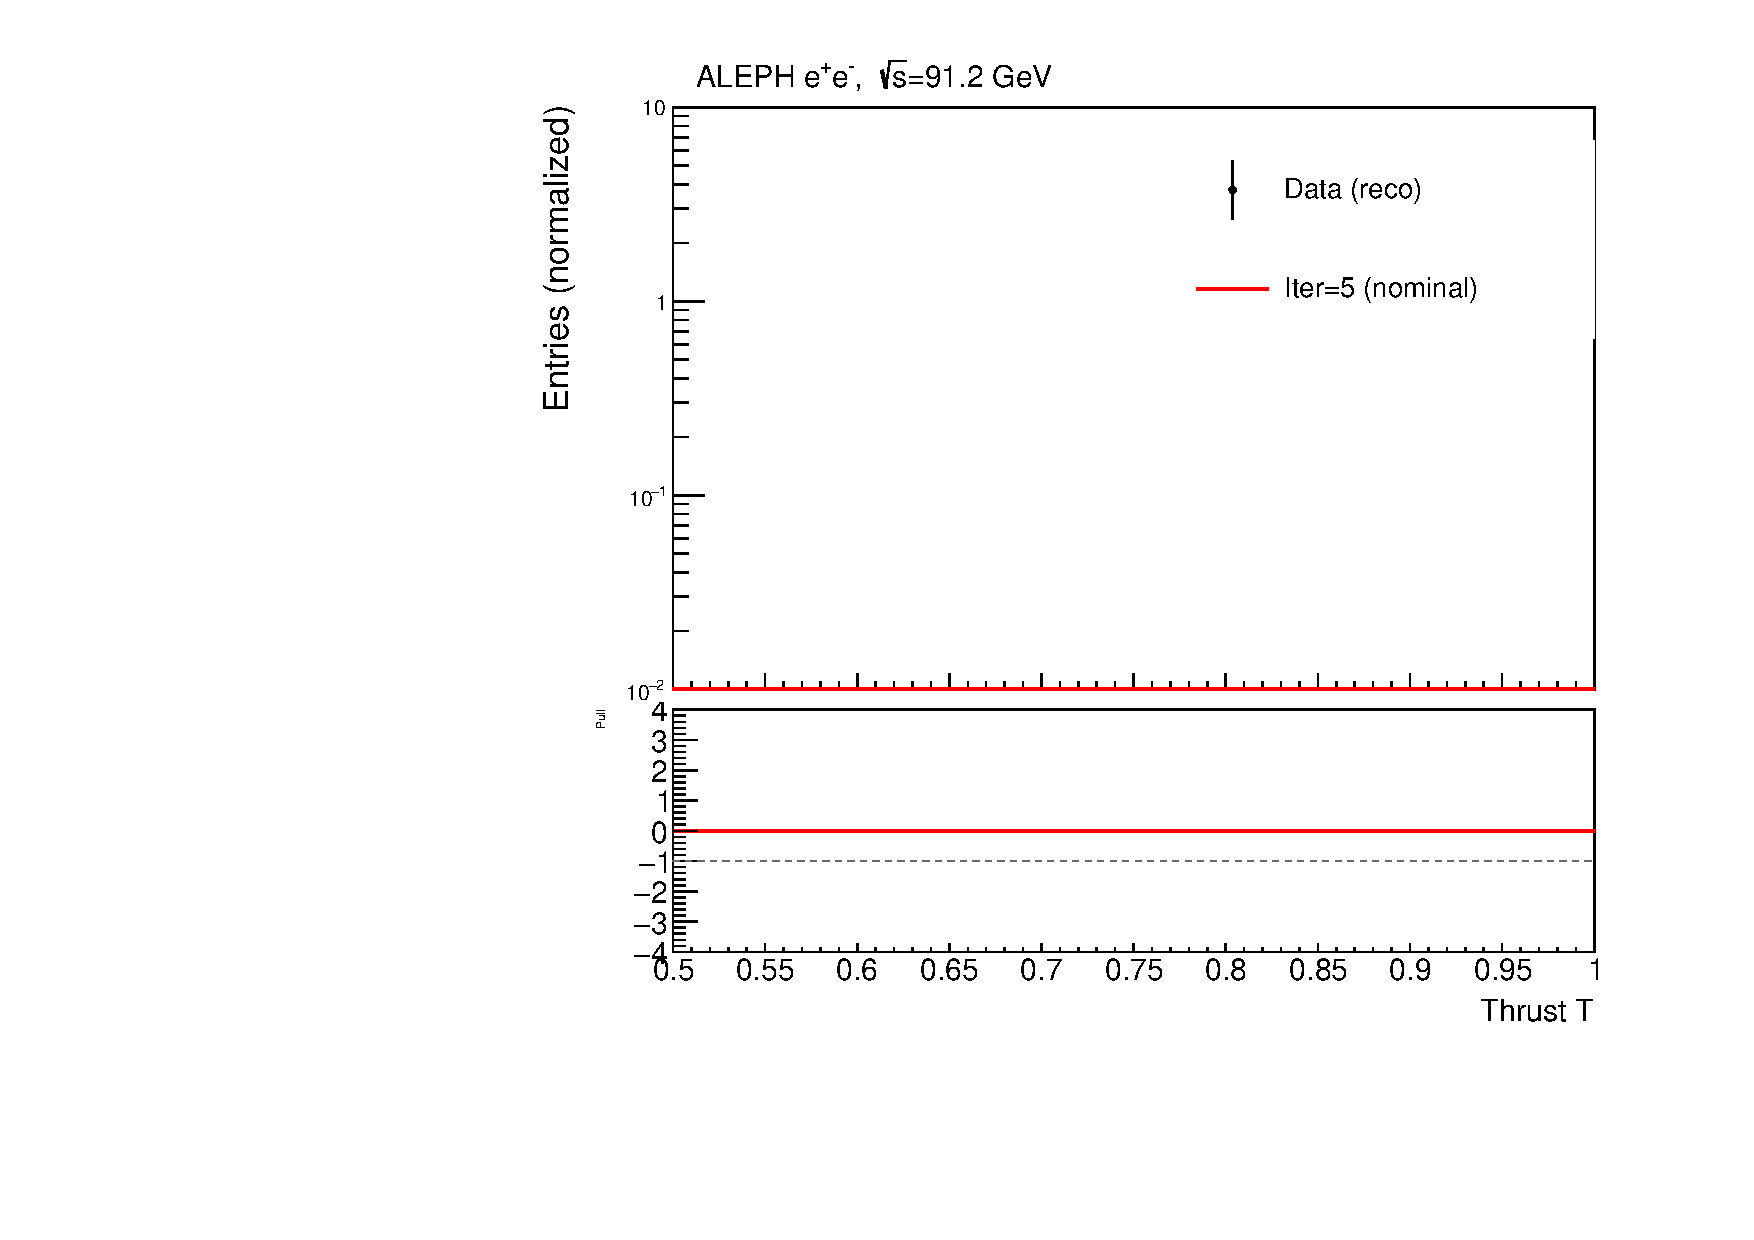
\includegraphics[width=0.65\textwidth]{../Studies/Phase2_Checks_2026-03-03/plots/pull_panel/dist_refolded_vs_data_pull.pdf}
\caption{Pull panel for refolded spectra: per-bin pull $(N_{\mathrm{data}} - N_{\mathrm{refold}})/\sigma$ for selected iteration points, showing bin-by-bin agreement between the detector-level data and each refolded prediction. Produced by \texttt{refolding\_pull\_panel.py} (see \texttt{Studies/Phase2\_Checks\_2026-03-03/}).}
\label{fig:refold_pull_panel}
\end{figure}

\begin{figure}[t!]
\centering
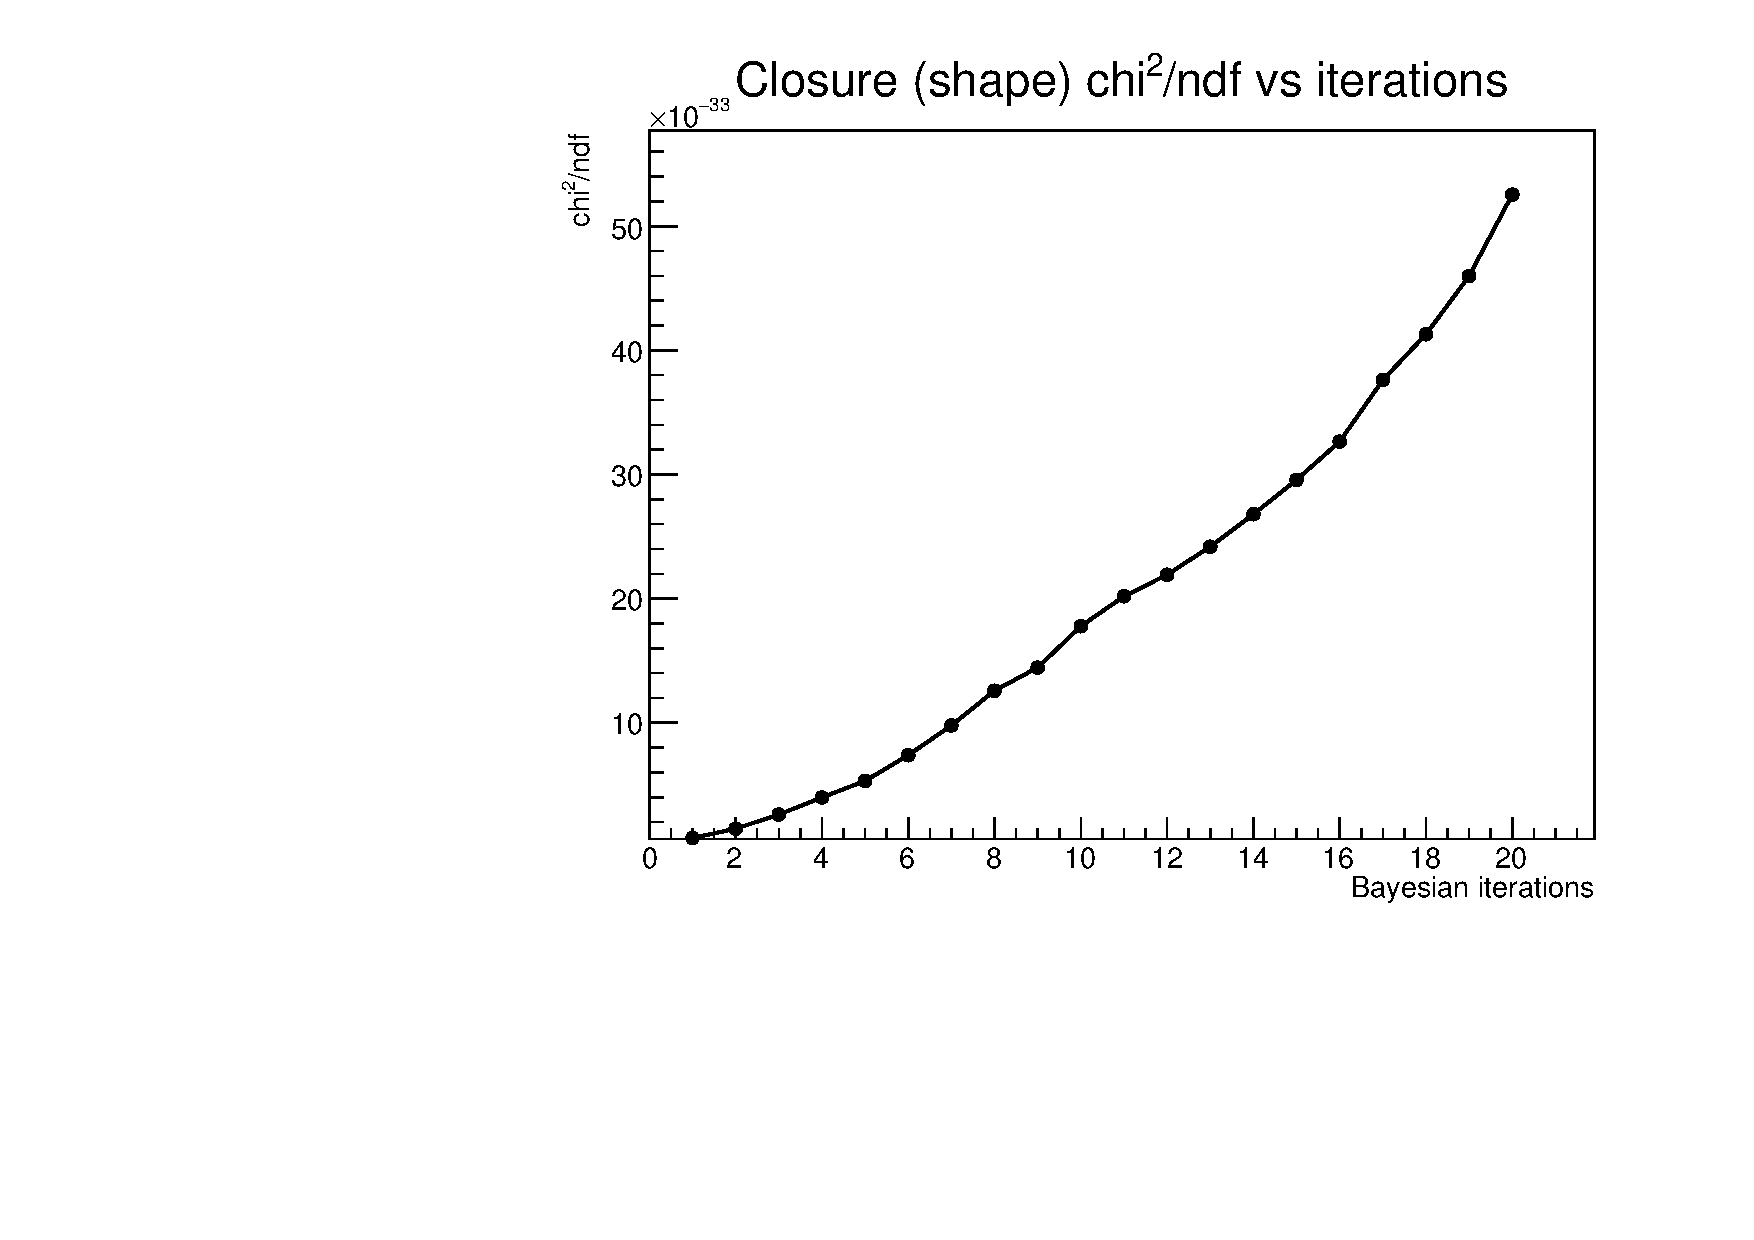
\includegraphics[width=0.49\textwidth]{../Studies/PreliminaryResult/2026-02-17_thrust_iter5/validation/iteration_scan/chi2ndf_closure_shape_vs_iterations.pdf}
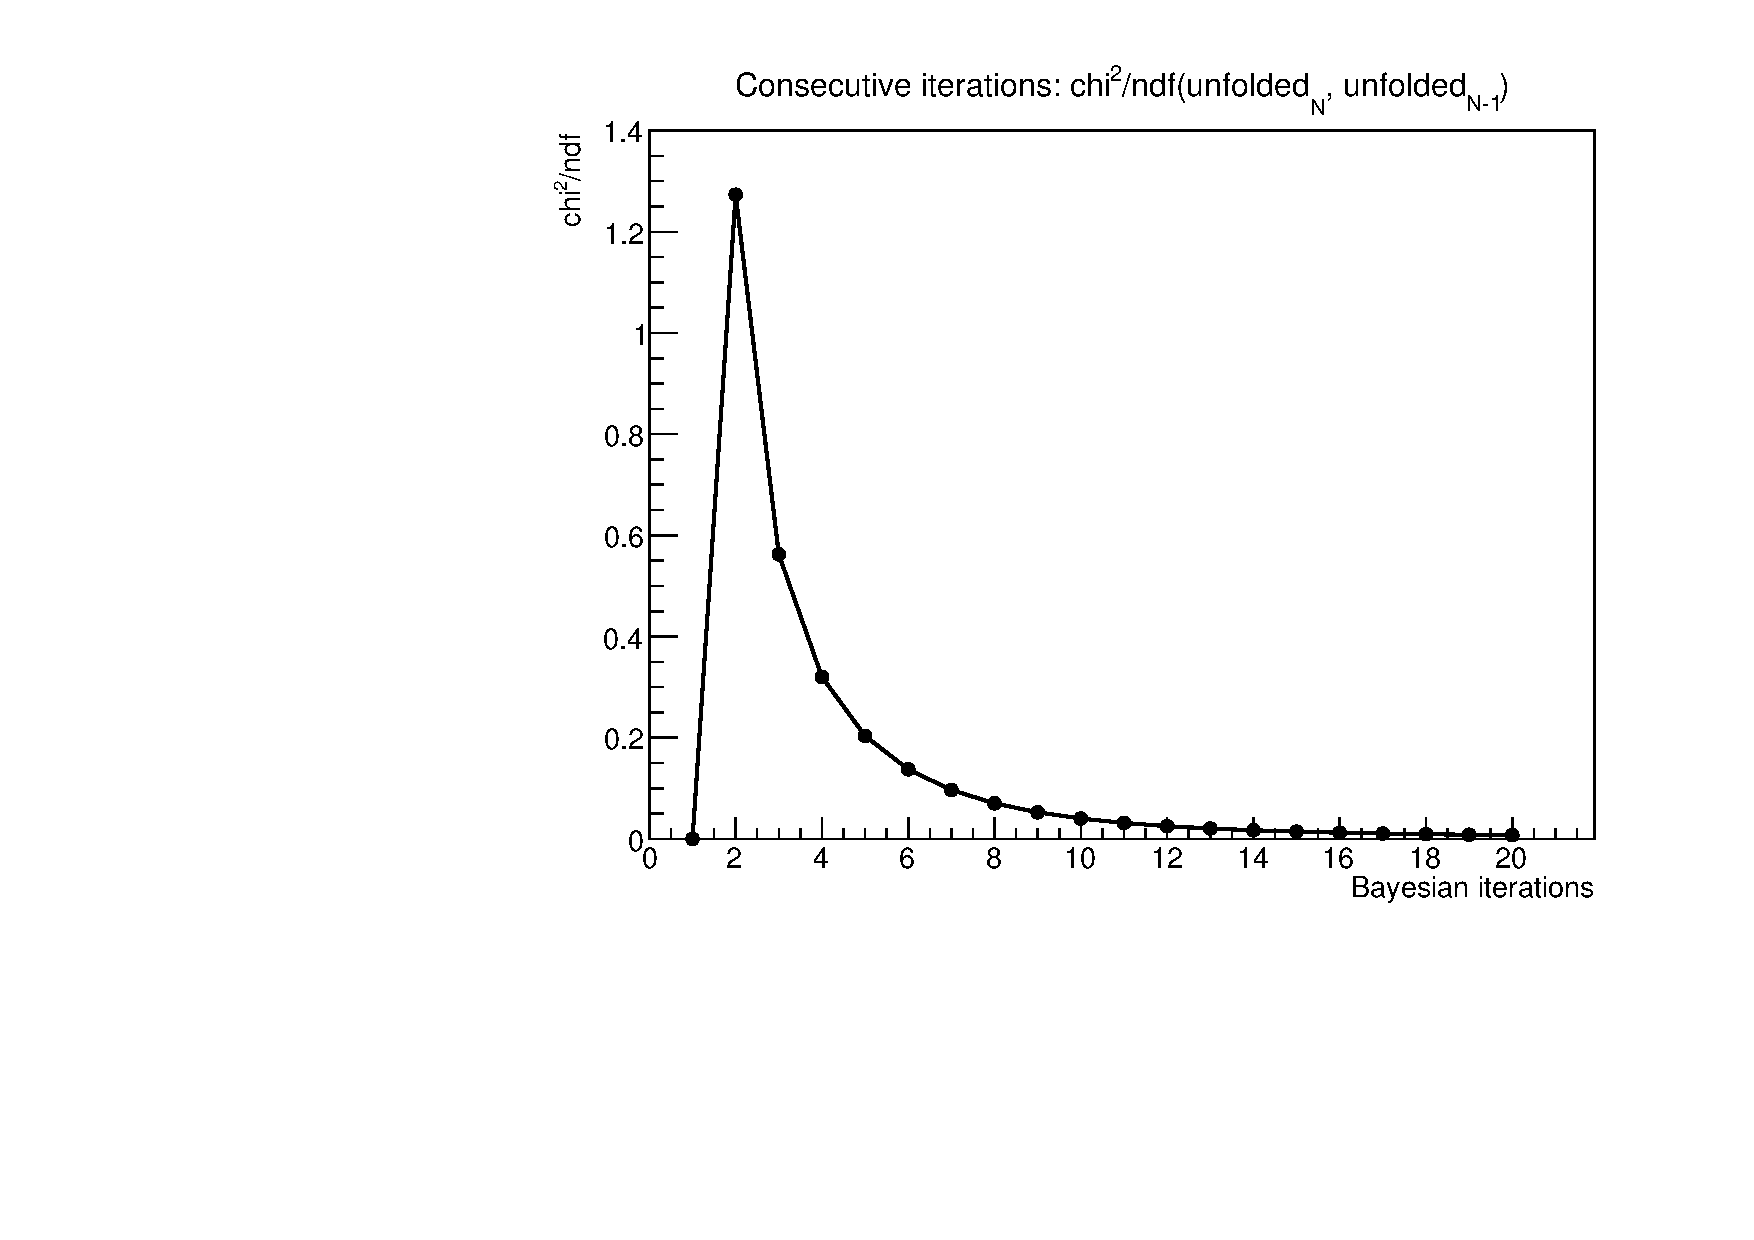
\includegraphics[width=0.49\textwidth]{../Studies/PreliminaryResult/2026-02-17_thrust_iter5/validation/iteration_scan/chi2ndf_iter_delta_counts_vs_iterations.pdf}
\\[2mm]
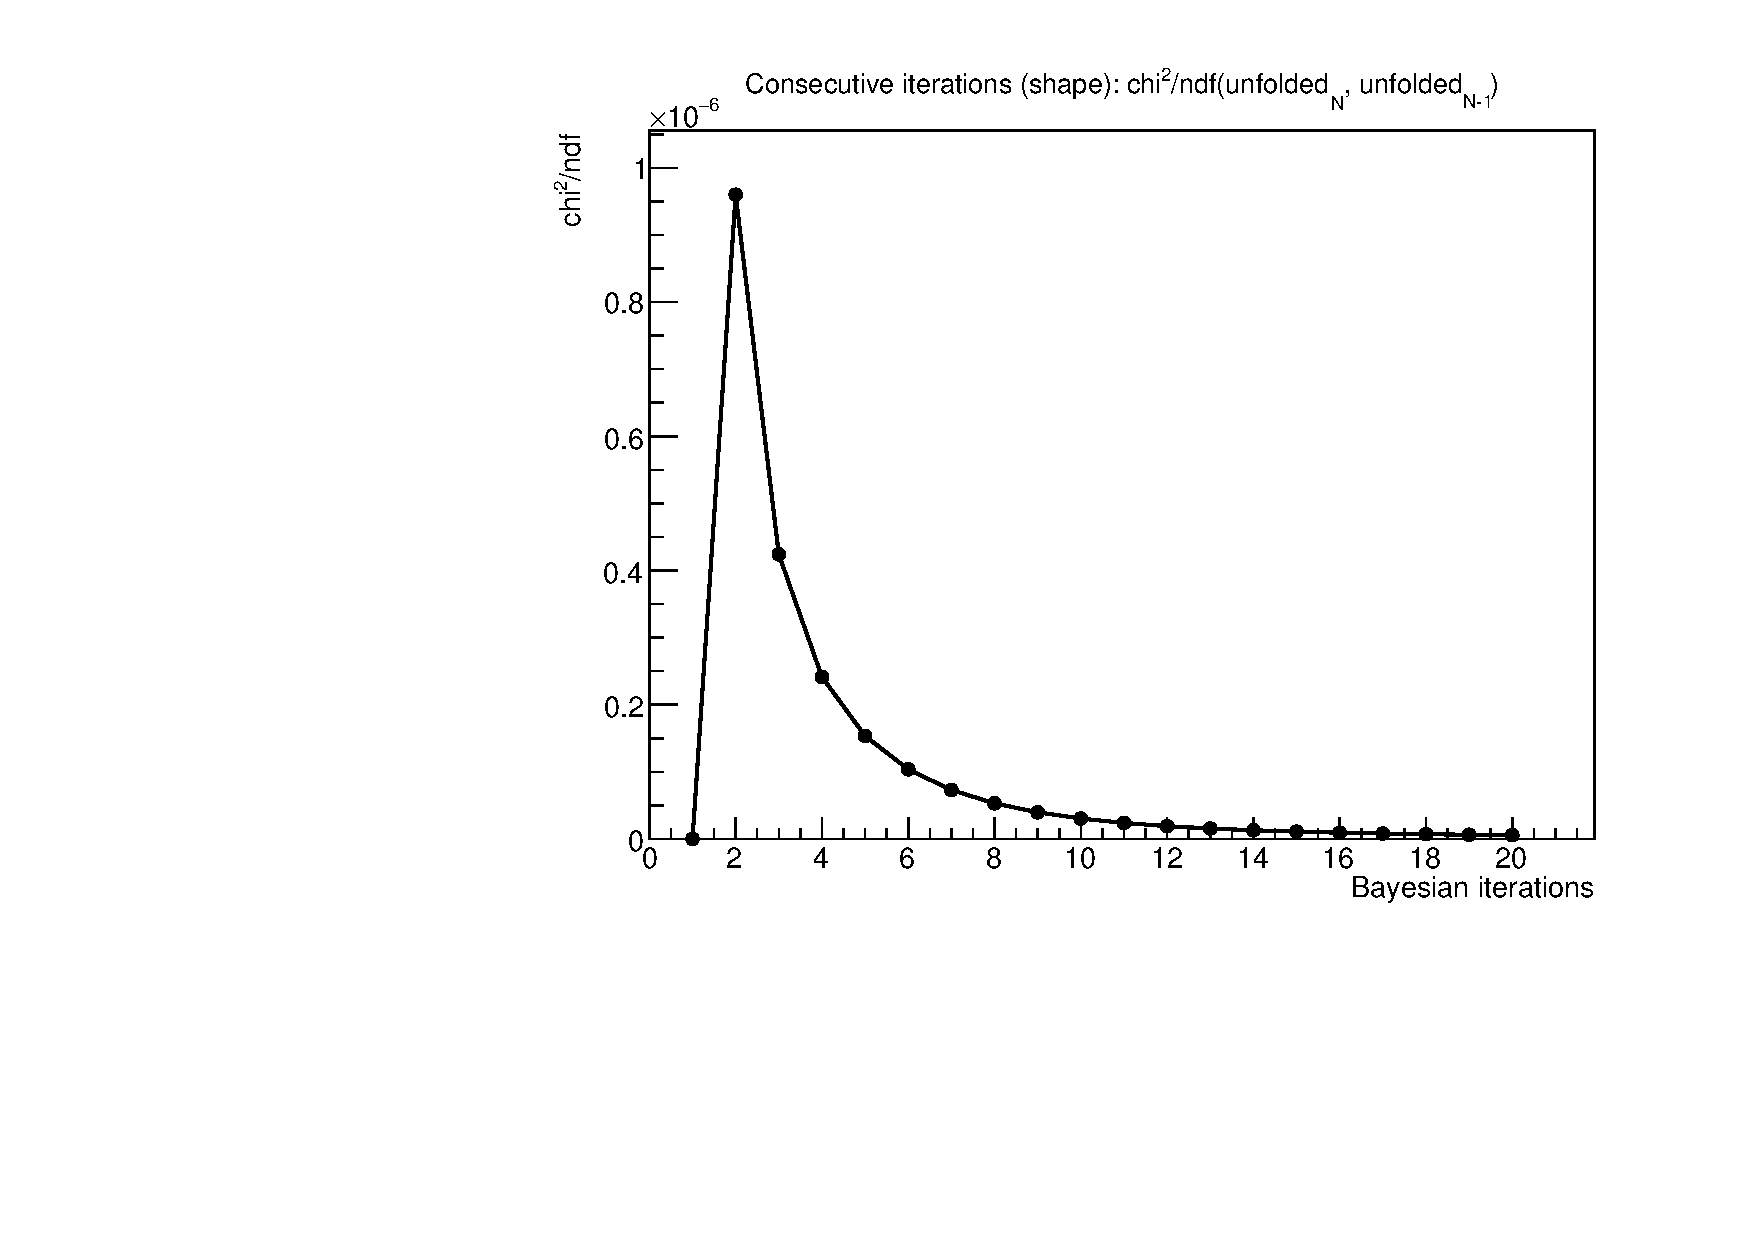
\includegraphics[width=0.49\textwidth]{../Studies/PreliminaryResult/2026-02-17_thrust_iter5/validation/iteration_scan/chi2ndf_iter_delta_shape_vs_iterations.pdf}
\caption{Iteration-choice diagnostics: closure-shape $\chi^2/\mathrm{ndf}$ (top left), iteration-to-iteration count-level stability (top right), and iteration-to-iteration shape stability (bottom left).}
\label{fig:iteration_choice_diagnostics}
\end{figure}

\FloatBarrier

\subsection{Thrust resolution study}
\label{sec:thrust_resolution}

The usable binning resolution varies across the thrust spectrum. To quantify this,
we use the matched reco--gen event pairs to study the thrust resolution as a function
of true thrust. Specifically, we plot $(T_{\mathrm{reco}} - T_{\mathrm{gen}})$ versus
$T_{\mathrm{gen}}$ in a two-dimensional histogram, and extract the resolution
$\sigma(T)$ as a function of $T_{\mathrm{gen}}$ from the per-slice width of the
$(T_{\mathrm{reco}} - T_{\mathrm{gen}})$ distribution. This study is particularly
important in the high-thrust (low $\tau = 1-T$) regime, which spans the peak of the
thrust distribution and the deep non-perturbative region. The previous ALEPH
analyses~\cite{Heister:2003aj} chose bin sizes to be ``somewhat smaller than twice
the corresponding detector resolution,'' and our IBU approach, while less sensitive
to binning than the matrix method, still uses this principle to guide the finest
bins tested in the region.

\begin{figure}[t!]
\centering
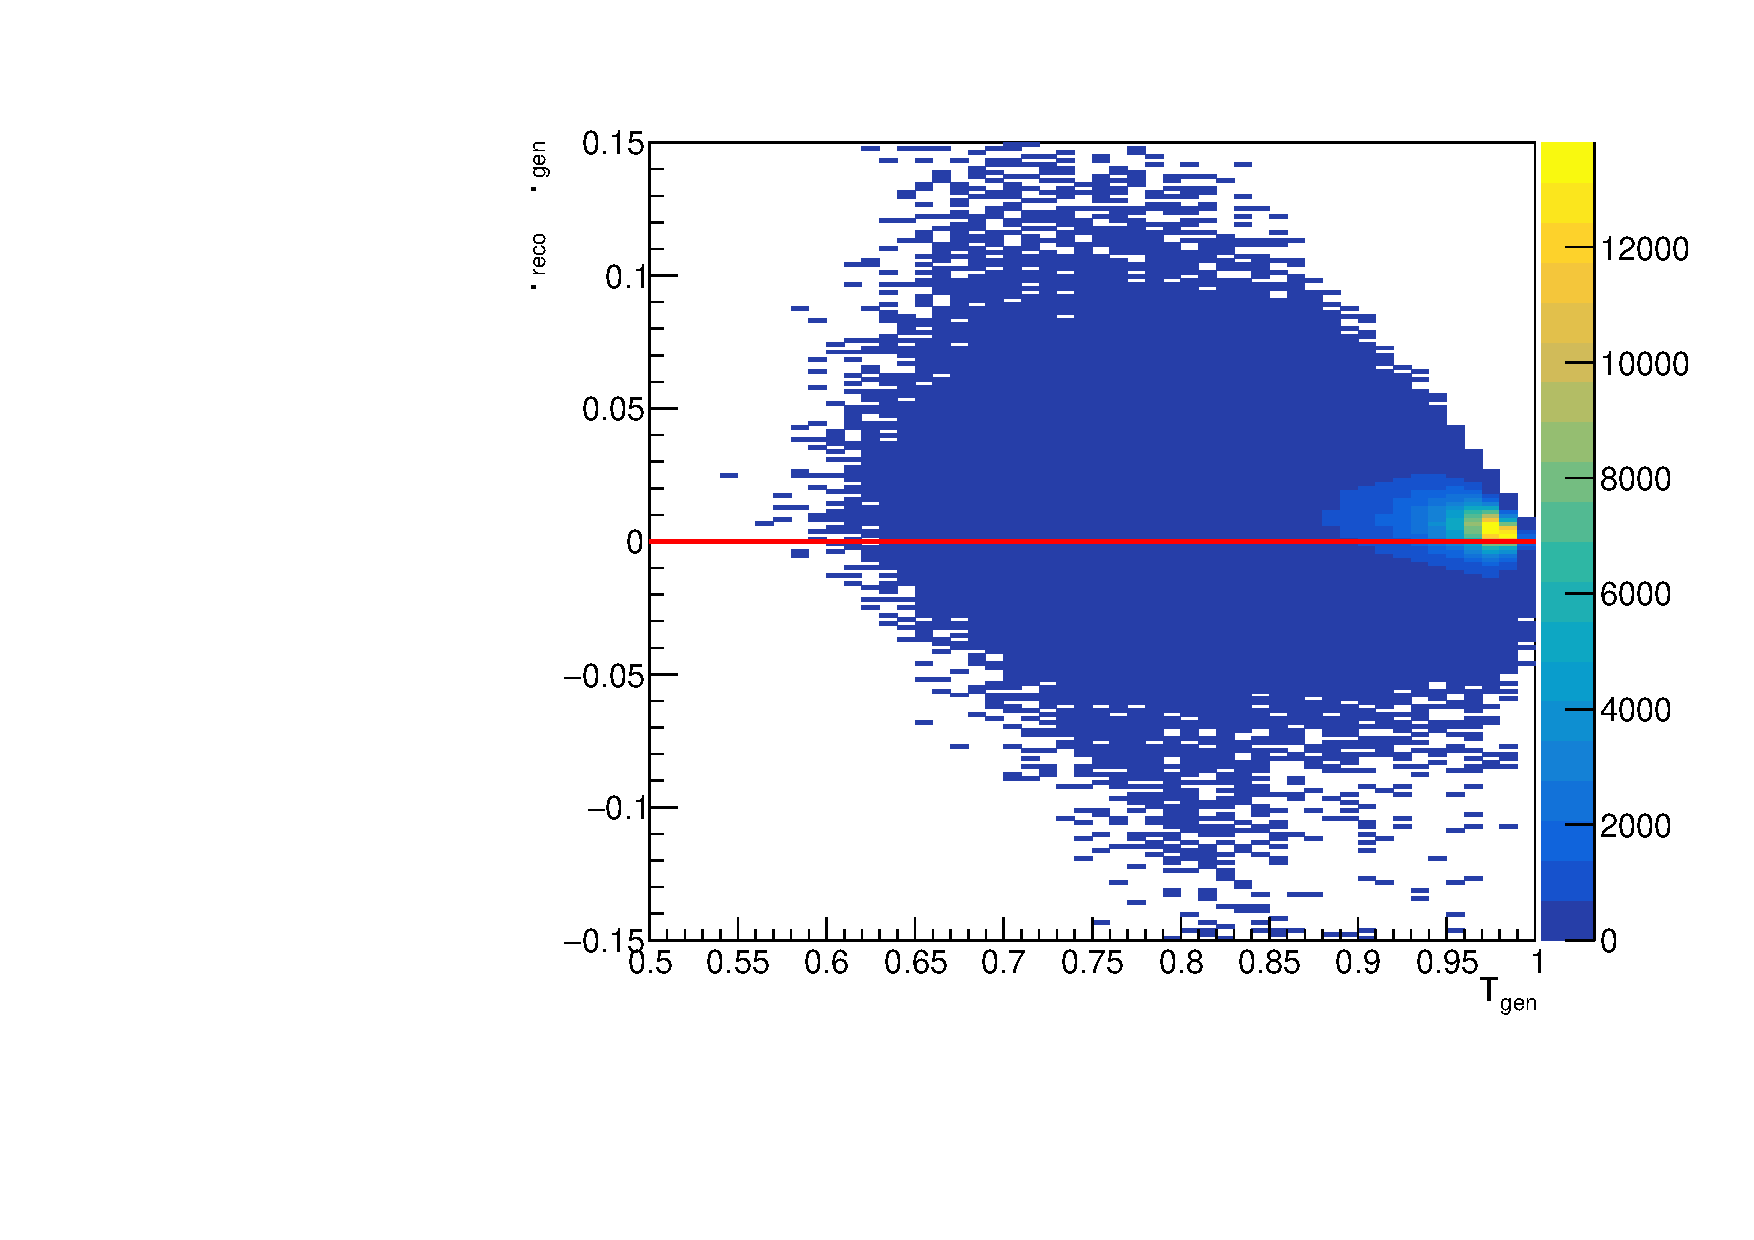
\includegraphics[width=0.60\textwidth]{../Studies/Phase2_Checks_2026-03-03/plots/thrust_resolution/thrust_resolution_2d.pdf}
\caption{Two-dimensional distribution of $(T_{\mathrm{reco}}-T_{\mathrm{gen}})$ vs $T_{\mathrm{gen}}$ for matched MC event pairs. The spread narrows toward $T\to1$ (low-$\tau$ region), motivating finer binning there.}
\label{fig:thrust_resolution_2d}
\end{figure}

\begin{figure}[t!]
\centering
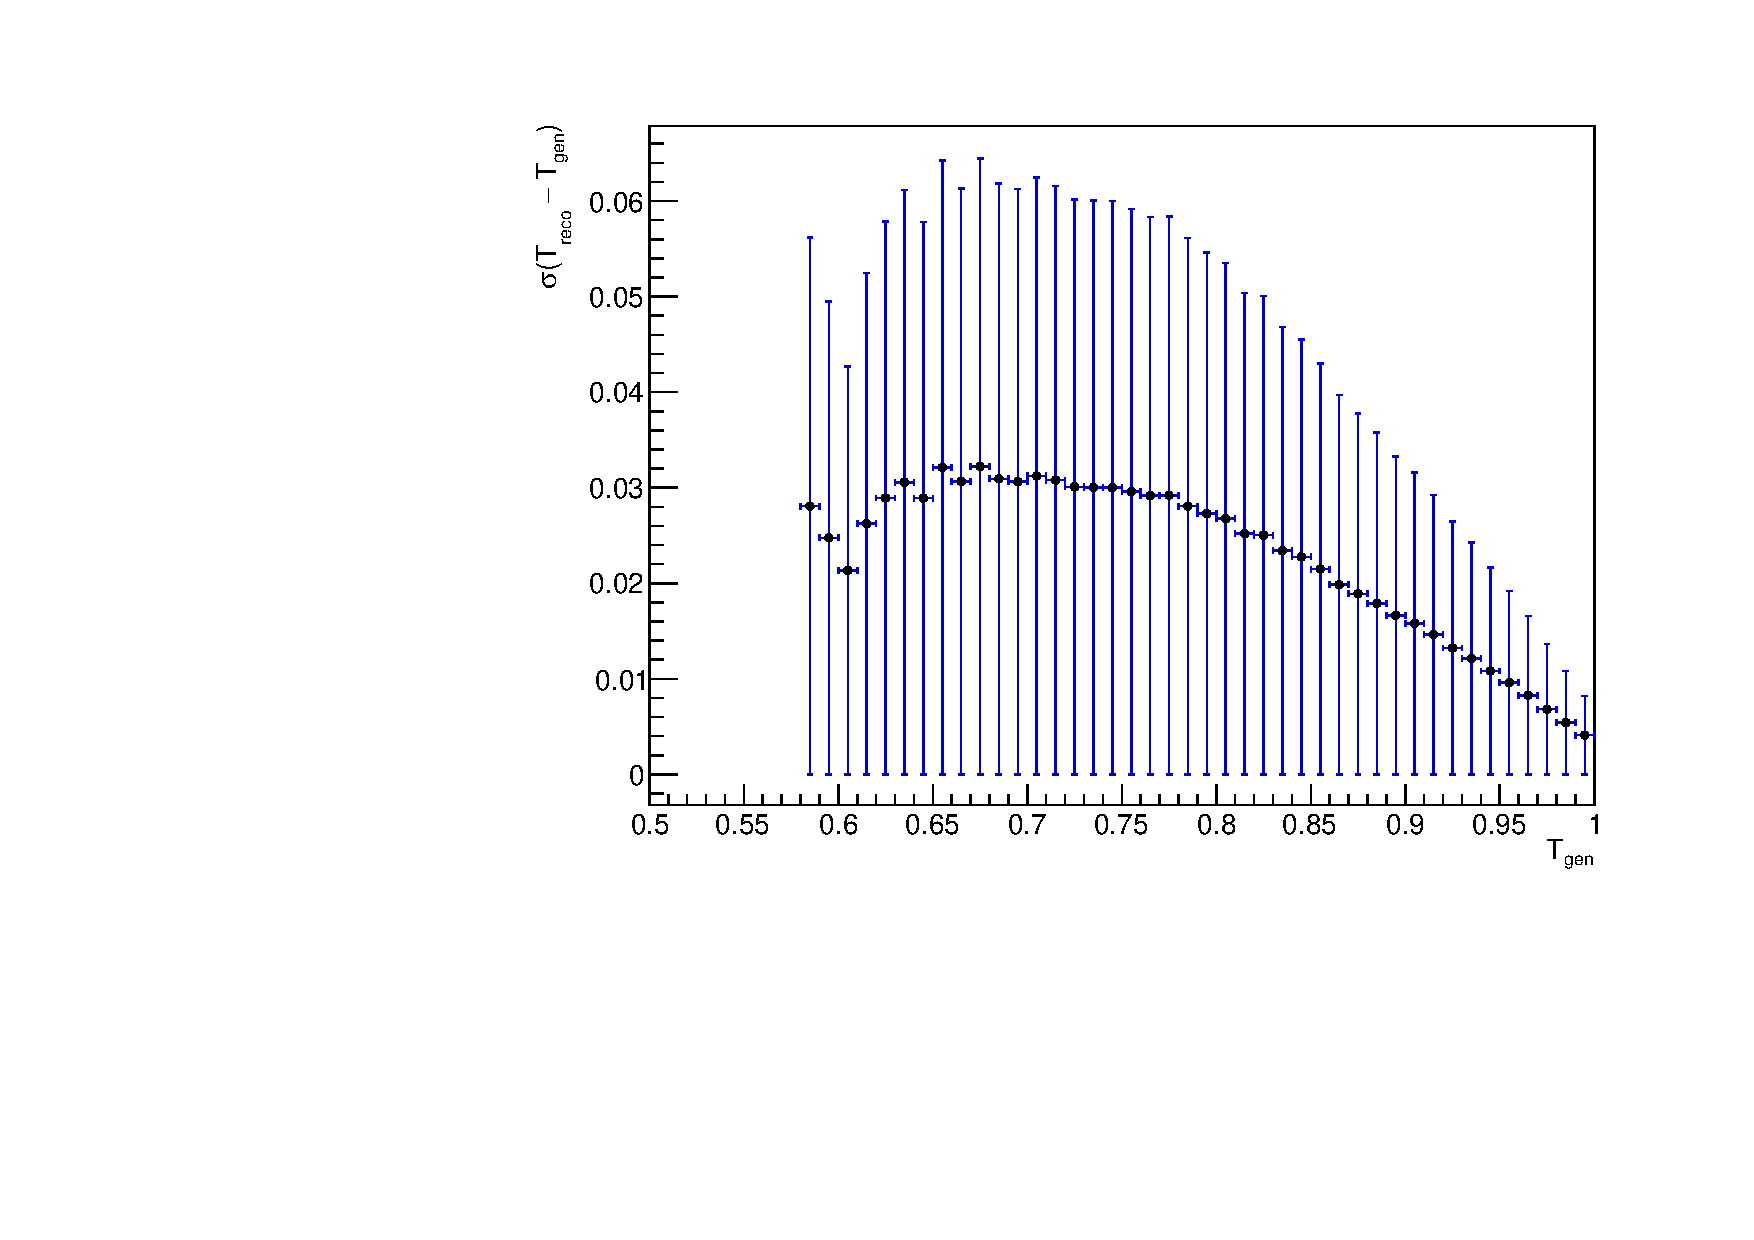
\includegraphics[width=0.49\textwidth]{../Studies/Phase2_Checks_2026-03-03/plots/thrust_resolution/thrust_resolution_profile.pdf}
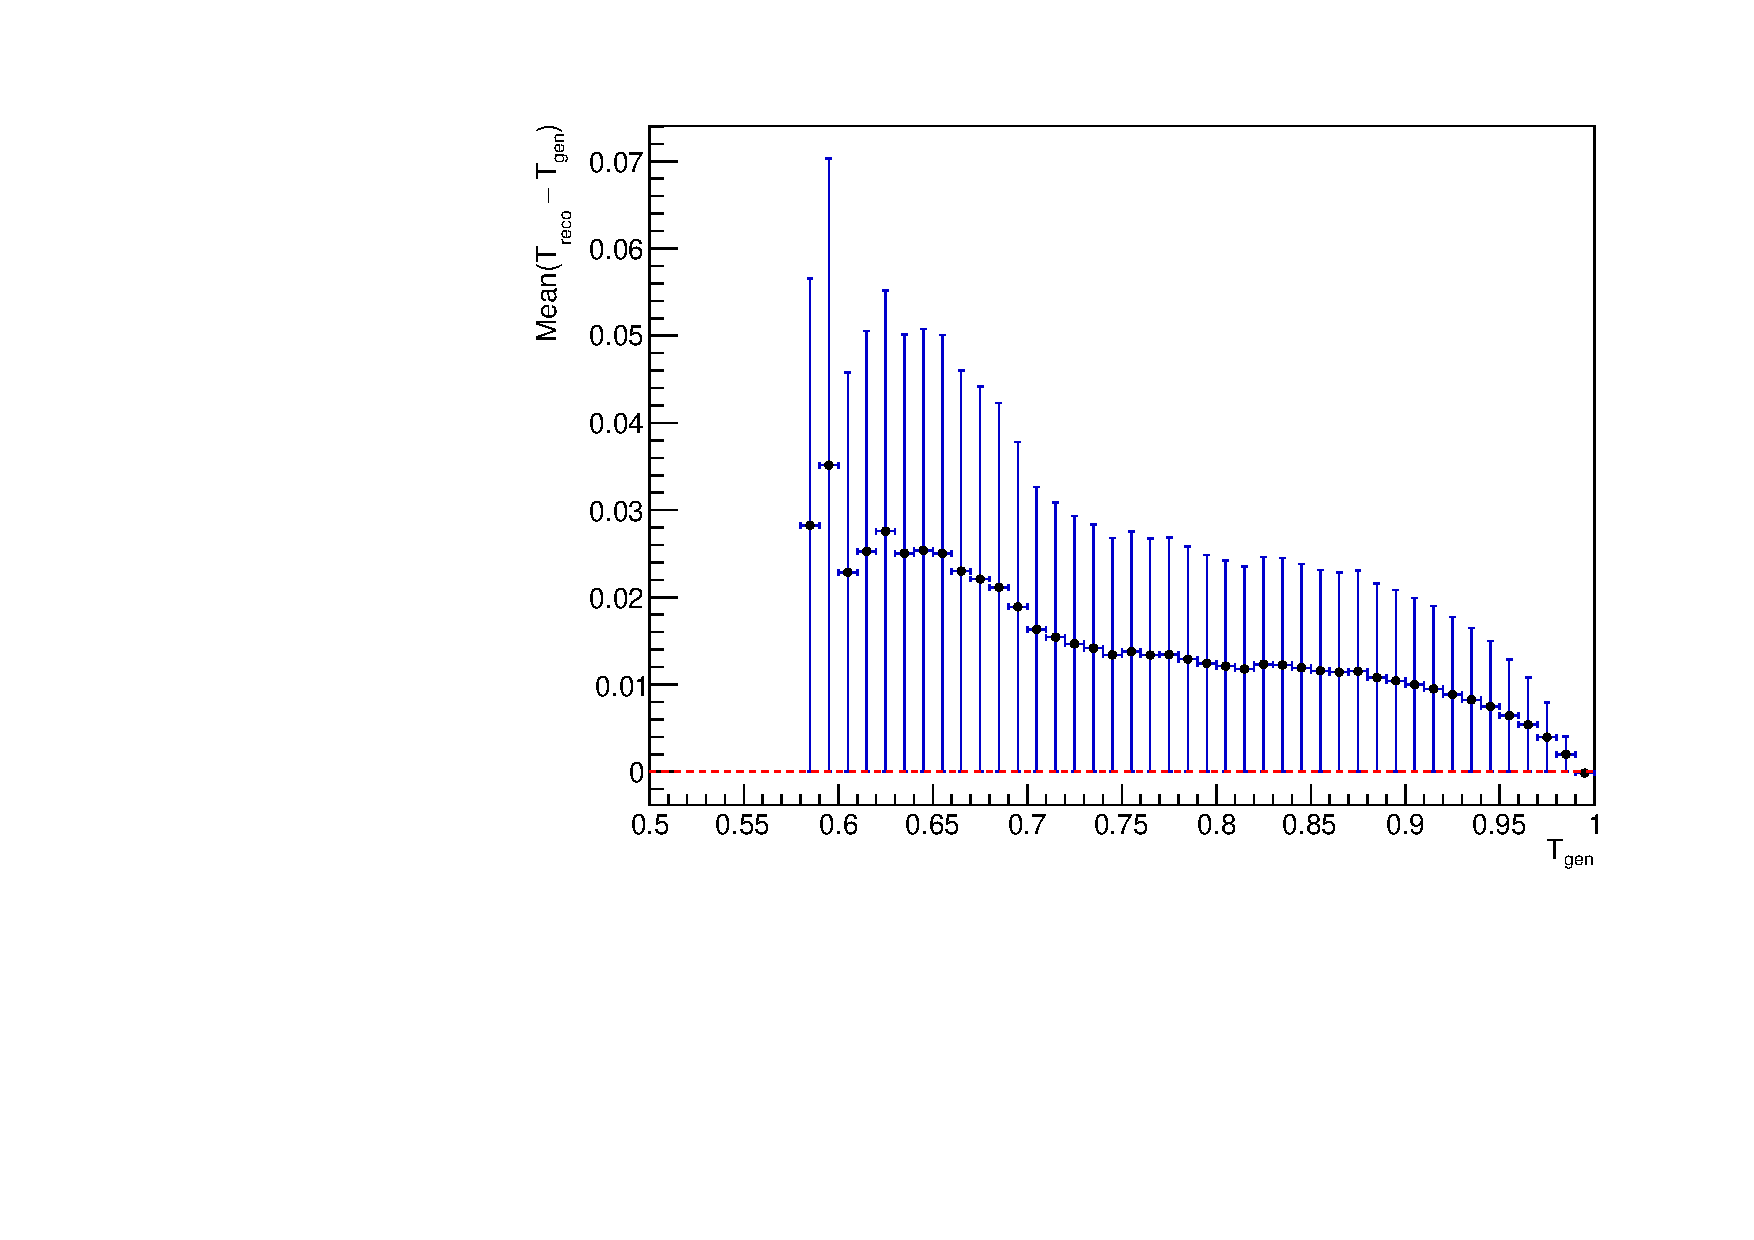
\includegraphics[width=0.49\textwidth]{../Studies/Phase2_Checks_2026-03-03/plots/thrust_resolution/thrust_resolution_bias.pdf}
\caption{Left: per-slice RMS of $(T_{\mathrm{reco}}-T_{\mathrm{gen}})$ as a function of $T_{\mathrm{gen}}$, giving the thrust resolution profile $\sigma(T)$. Right: mean bias $\langle T_{\mathrm{reco}}-T_{\mathrm{gen}}\rangle$ vs $T_{\mathrm{gen}}$; values consistent with zero indicate no systematic shift.}
\label{fig:thrust_resolution_profile}
\end{figure}

\subsection{Systematics execution map}

Systematic branches are executed by rerunning unfolding with variation-specific inputs or theory weights, then converting each branch into a signed shift relative to nominal.
The combination structure is summarized in Table~\ref{fig:systematics_execution_chart}.

\begin{figure}[t!]
\centering
\resizebox{0.98\linewidth}{!}{%
\begin{tikzpicture}[
  >=Latex,
  node distance=6mm,
  every node/.style={font=\footnotesize},
  block/.style={draw, rounded corners, align=left, text width=5.5cm, inner sep=4pt},
  merge/.style={draw, rounded corners, align=center, text width=7.2cm, inner sep=4pt},
  diag/.style={draw, rounded corners, align=left, text width=5.5cm, inner sep=4pt, dashed},
  arrow/.style={-Latex, line width=0.8pt}
]

\node[block] (iter) {\textbf{Iteration component}\newline
Inputs: \texttt{iter4}, \texttt{iter6}\newline
Rule: envelope per bin};

\node[block, right=11mm of iter] (track) {\textbf{Track/event component}\newline
Inputs: \texttt{ntpc7}, \texttt{pt04}, \texttt{ech10}, \texttt{with\_met}\newline
Rule: quadrature of absolute shifts};

\node[block, right=11mm of track] (neutral) {\textbf{Neutral component}\newline
Inputs: \texttt{nes\_up}, \texttt{nes\_down}, \texttt{ner}\newline
Rule: NES envelope, then quadrature with NER};

\node[block, below=7mm of track] (theory) {\textbf{Theory component}\newline
Inputs: \texttt{pythia8}, \texttt{herwig}, \texttt{sherpa}\newline
Rule: envelope across generators};

\node[diag, left=11mm of theory] (noneu) {\textbf{Cross-check branch}\newline
Input: \texttt{no\_neutrals}\newline
Diagnostic only (excluded from total)};

\node[merge, right=11mm of theory] (total) {\textbf{Total uncertainty model}\newline
$\Delta_{\mathrm{tot}}=\sqrt{\Delta_{\mathrm{stat}}^2+\Delta_{\mathrm{iter}}^2+\Delta_{\mathrm{exp}}^2+\Delta_{\mathrm{theory}}^2}$\newline
with $\Delta_{\mathrm{exp}}=\sqrt{\Delta_{\mathrm{track/event}}^2+\Delta_{\mathrm{neutral}}^2}$};

\draw[arrow] (iter.south) -- ++(0,-4mm) -| (total.north west);
\draw[arrow] (track.south) -- ++(0,-4mm) -- (theory.north);
\draw[arrow] (neutral.south) -- ++(0,-4mm) -| (total.north east);
\draw[arrow] (theory.east) -- (total.west);
\draw[arrow, dashed] (noneu.east) -- (theory.west);

\end{tikzpicture}
}
\caption{Systematics combination chart for the thrust baseline. Solid arrows indicate components entering the nominal total uncertainty; dashed branch is the reported stress-test excluded from total.}
\label{fig:systematics_execution_chart}
\end{figure}


The nominal total uncertainty model (Sec.~\ref{sec:systematics}) combines component magnitudes in quadrature after branch-specific envelope or quadrature rules.
The \texttt{no\_neutrals} branch is retained as a stress-test and explicitly reported, but excluded from the nominal total.

\subsection{Hadronic correction, covariance propagation, and matrix exports}

After unfolding, a bin-wise hadronic event-selection correction is applied,
\begin{equation}
C_{\mathrm{had}}(j)=\frac{N_{\mathrm{genBefore}}(j)}{N_{\mathrm{gen}}(j)},
\qquad
U_j^{\mathrm{corr}} = U_j\,C_{\mathrm{had}}(j).
\end{equation}

For the nominal run, the statistical covariance is computed by RooUnfold using analytical error propagation (\texttt{RooUnfold::kCovariance}), which propagates Poisson uncertainties in the data and response histograms through the IBU iteration chain without toy MC sampling. The resulting covariance matrix is read from the unfolding output and transformed to the normalized differential-thrust basis used in this note. Non-statistical component covariances are built with a configurable model (nominal: \texttt{template\_correlated}), and fit-window covariance products are exported together with full-range matrices by
\texttt{build\_prelim\_uncertainty\_summary.py}.

Response and matrix visualizations are exported by the matrix-plot helper script (see Appendix~\ref{sec:app_workflow_code} for details). Full provenance metadata for the run, including git commit, ROOT version, RooUnfold version, environment fingerprint, response diagnostics, theory-weight coverage, and all computed uncertainty metrics, is written to a structured JSON summary file. This file is the primary machine-readable record of the result and is the canonical reference for any numeric claims in Sec.~\ref{sec:results}.

\begin{figure}[t!]
\centering
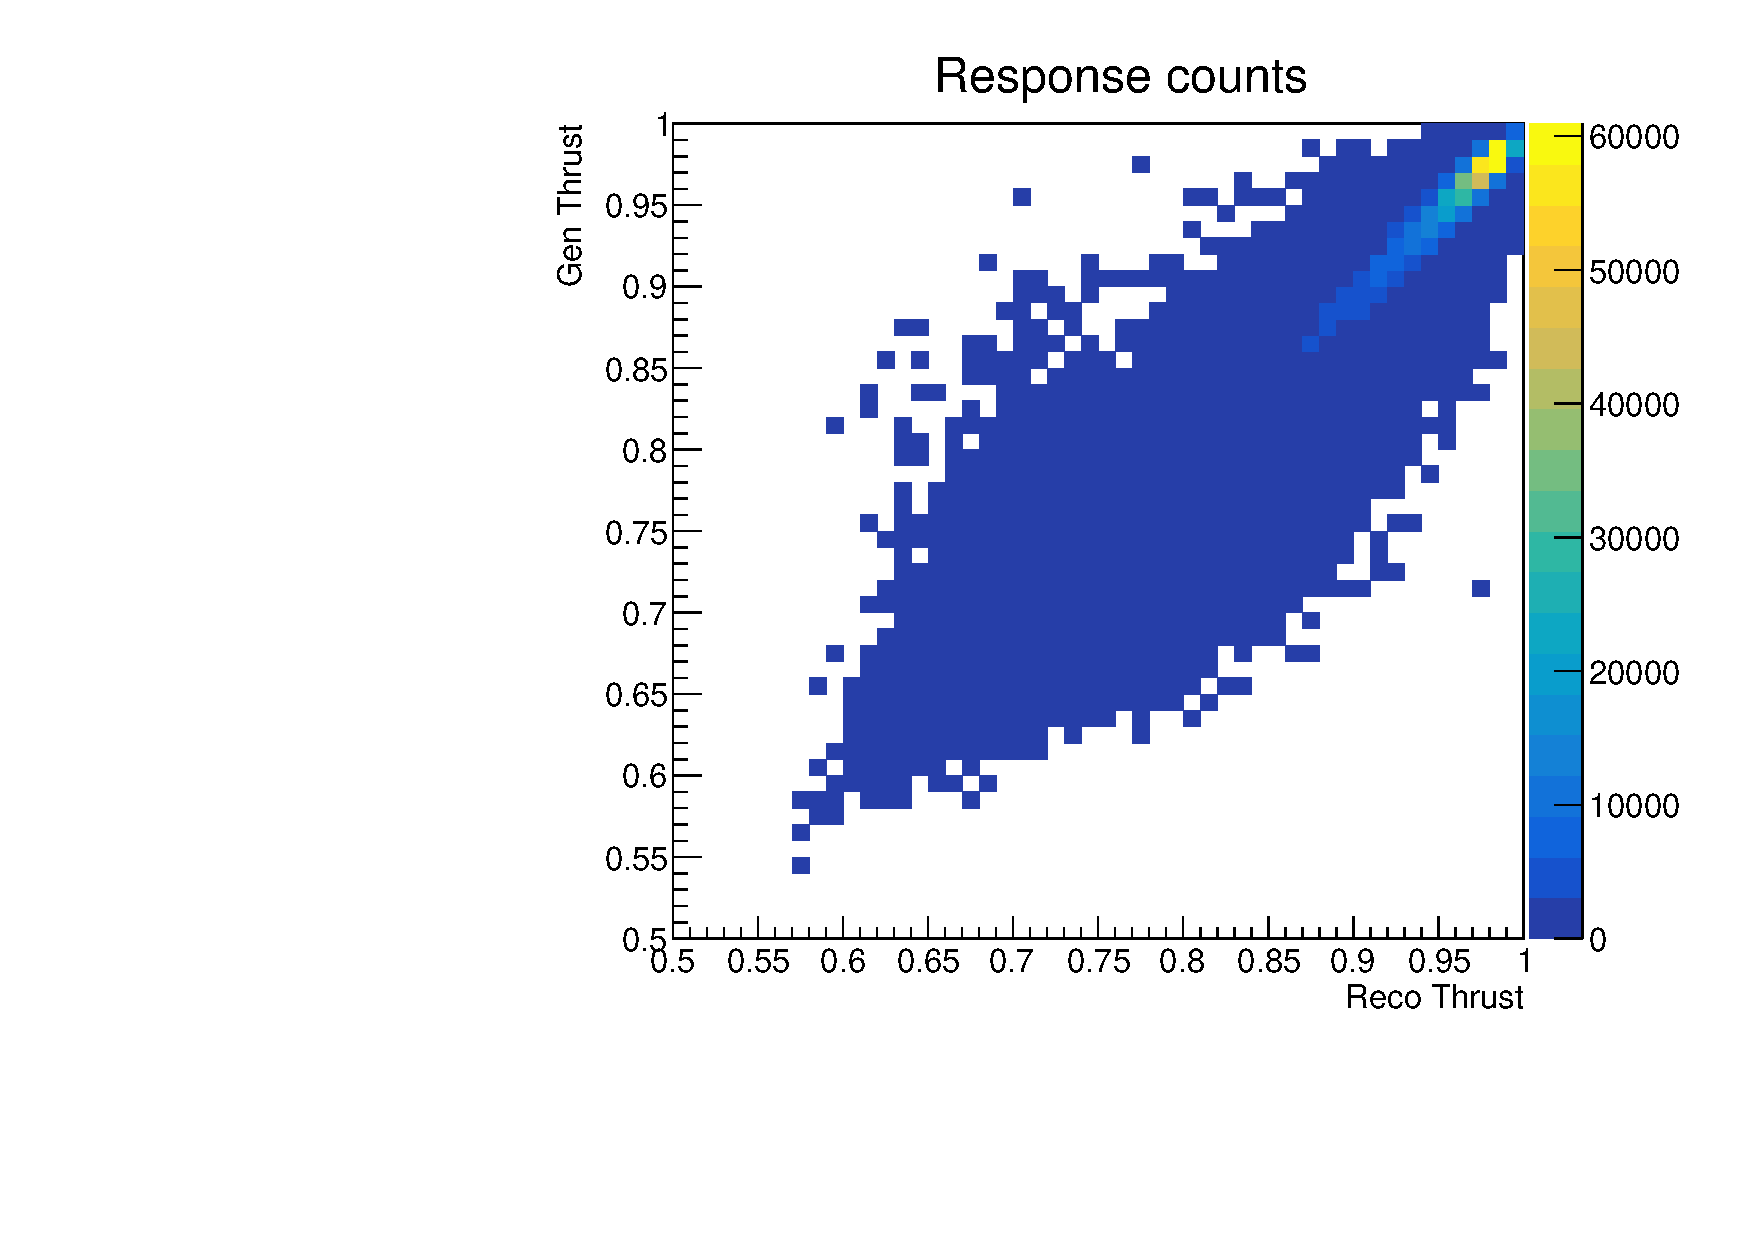
\includegraphics[width=0.49\textwidth]{../Studies/PreliminaryResult/2026-02-17_thrust_iter5/summary/matrices_nominal_iter5/matrix_response_counts.pdf}
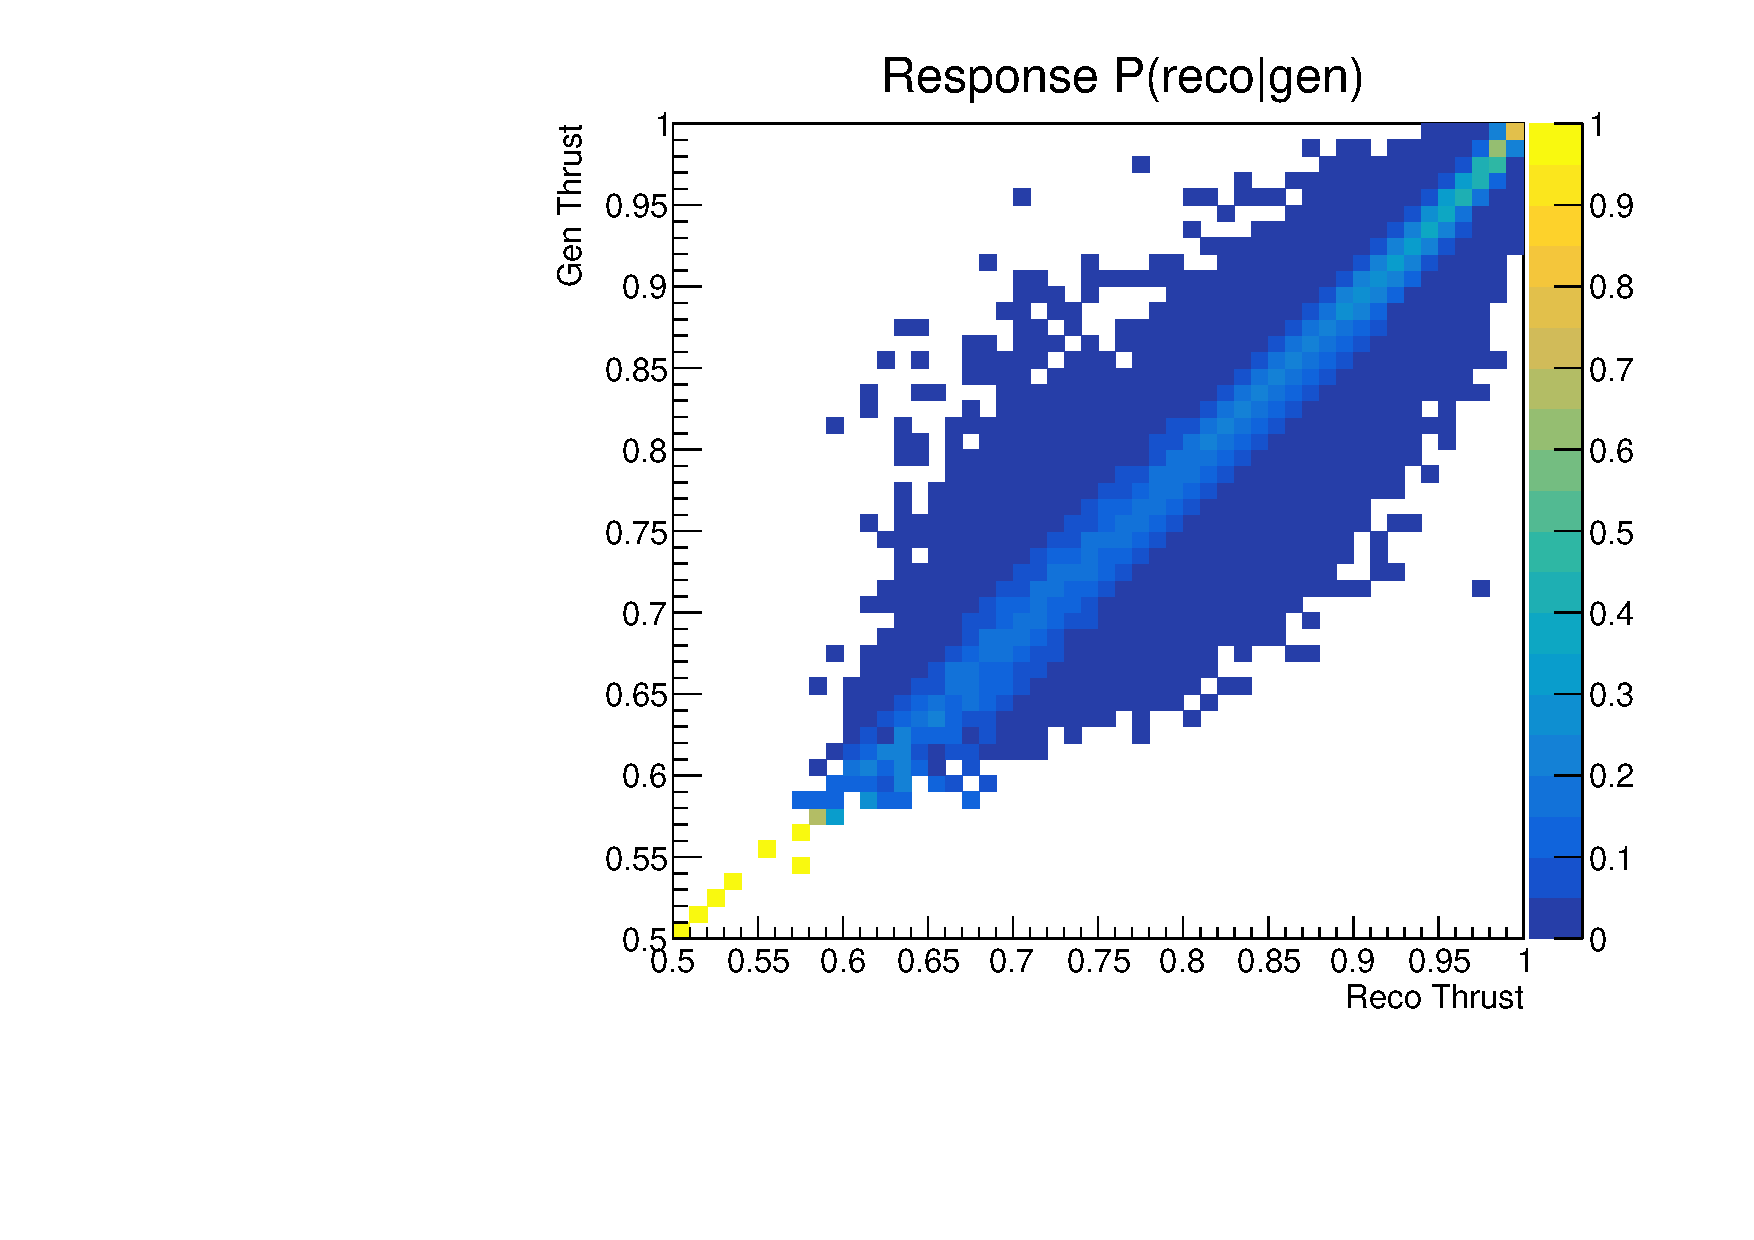
\includegraphics[width=0.49\textwidth]{../Studies/PreliminaryResult/2026-02-17_thrust_iter5/summary/matrices_nominal_iter5/matrix_response_probability.pdf}
\caption{Nominal response matrices for thrust: response counts (left) and response probability (right).}
\label{fig:response_matrices_nominal}
\end{figure}

\begin{figure}[t!]
\centering
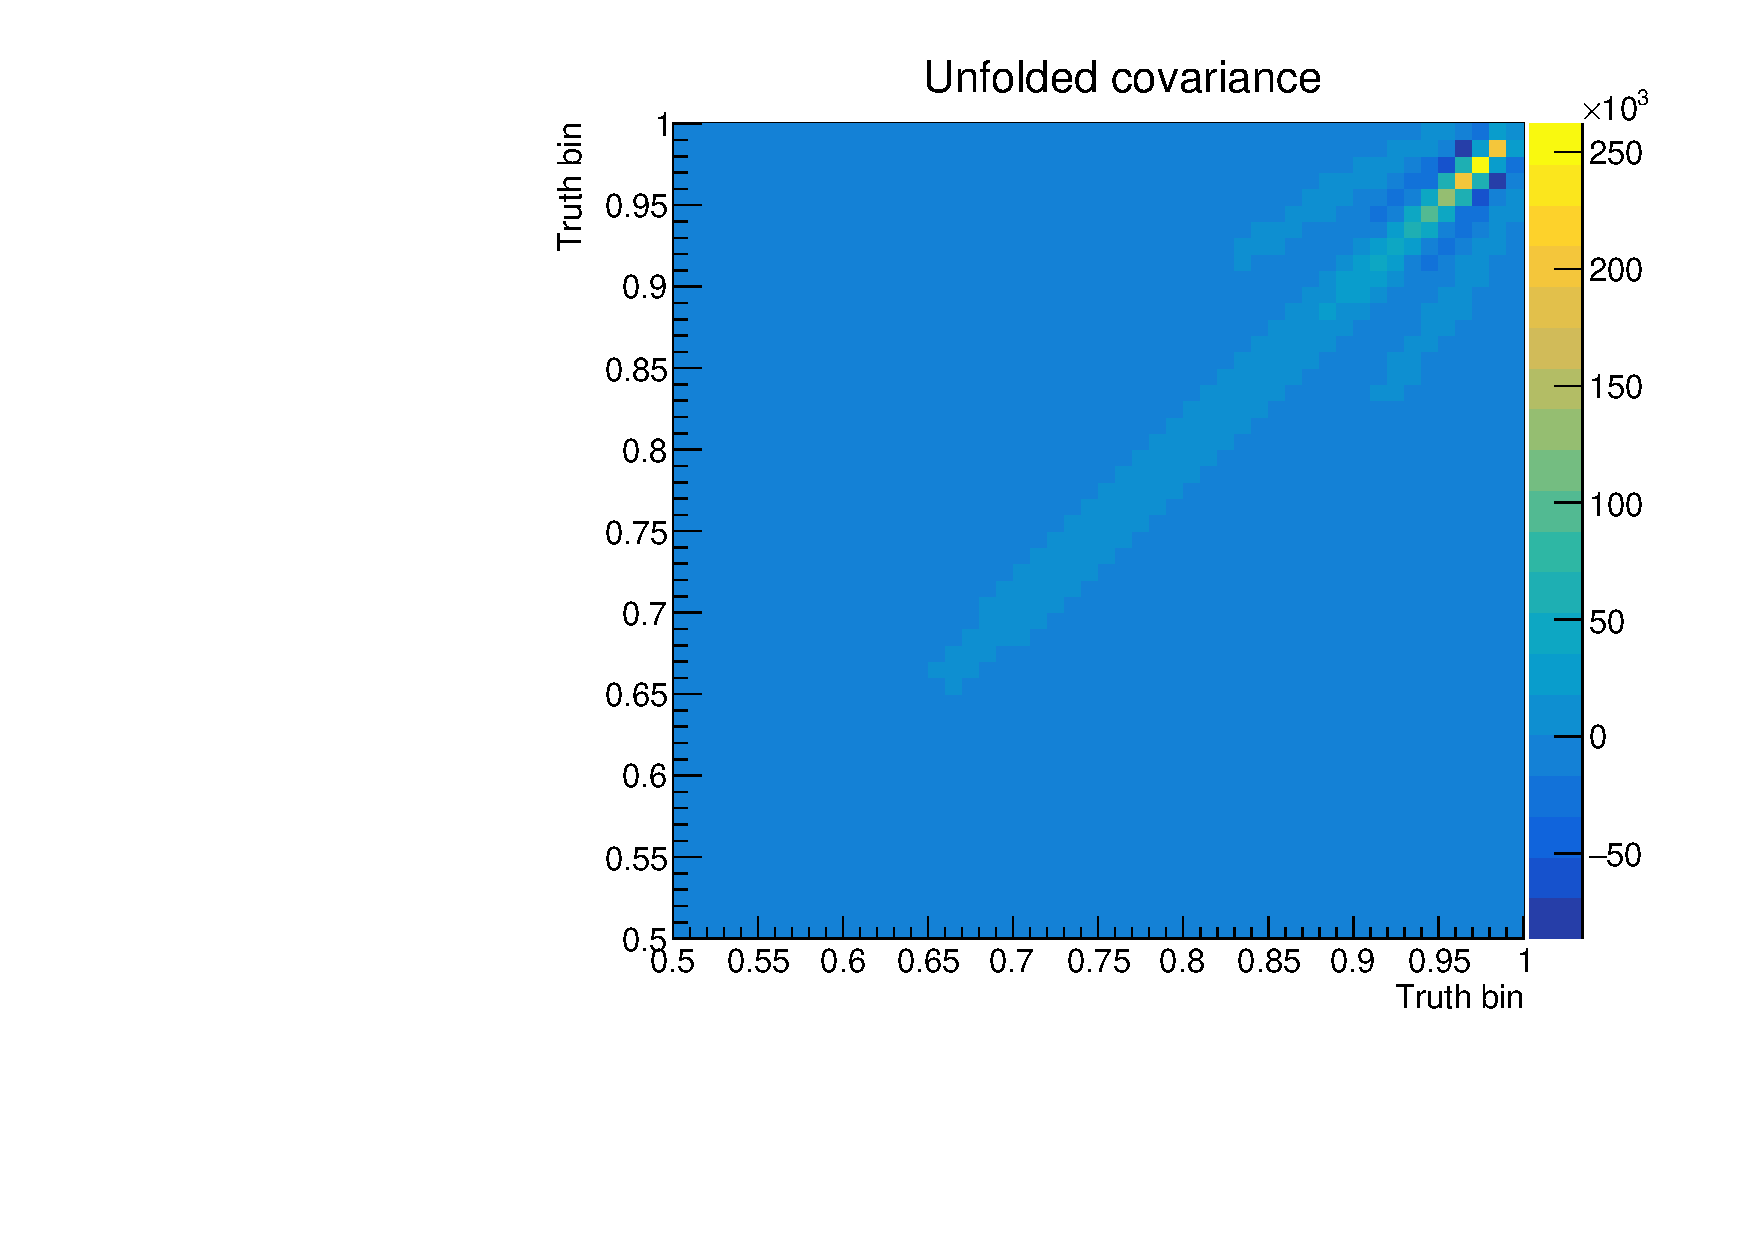
\includegraphics[width=0.49\textwidth]{../Studies/PreliminaryResult/2026-02-17_thrust_iter5/summary/matrices_nominal_iter5/matrix_unfold_covariance.pdf}
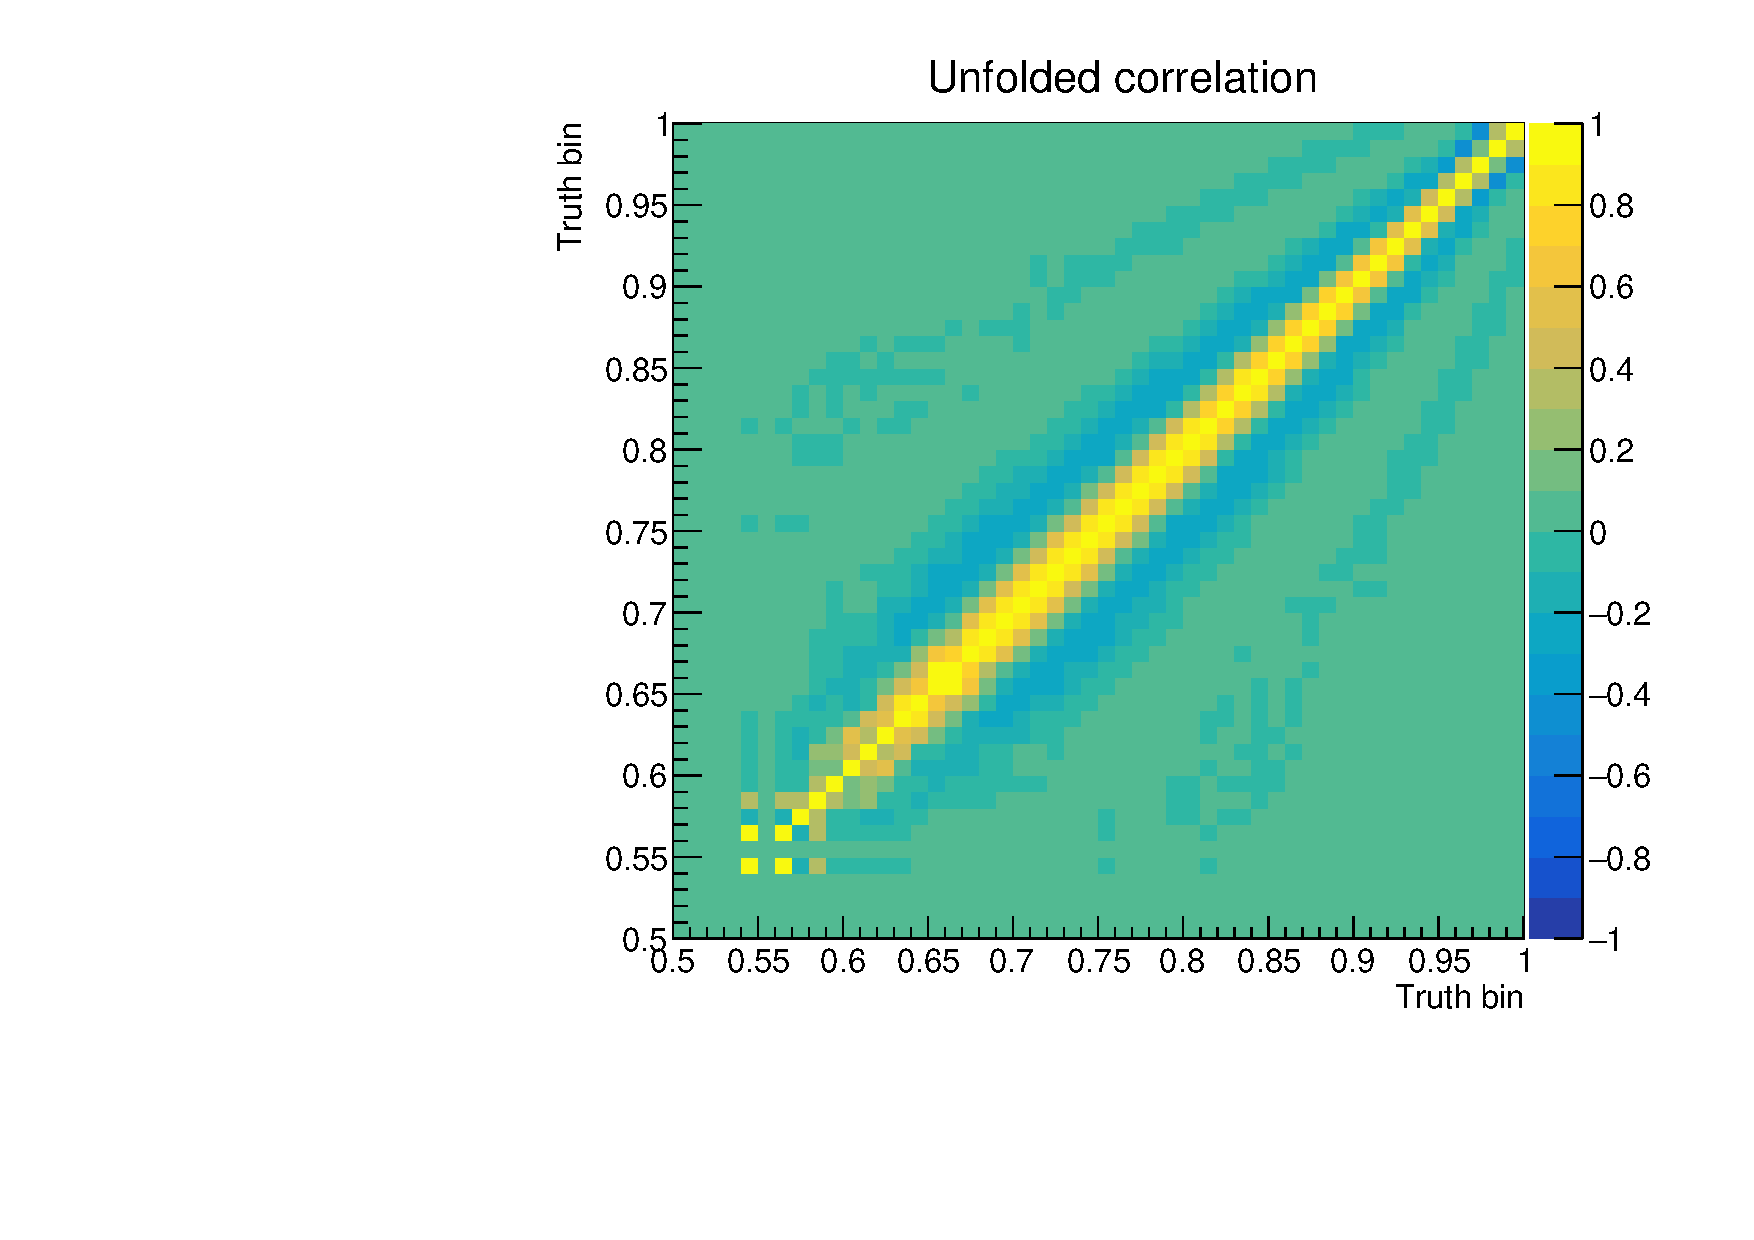
\includegraphics[width=0.49\textwidth]{../Studies/PreliminaryResult/2026-02-17_thrust_iter5/summary/matrices_nominal_iter5/matrix_unfold_correlation.pdf}
\caption{Nominal unfolded covariance matrix (left) and corresponding correlation matrix (right).}
\label{fig:covariance_correlation_nominal}
\end{figure}

The nominal and systematics execution logic, including command sequences, pseudocode for workflow control and uncertainty assembly, and the reproduction contract for this note, are documented in Appendix~\ref{sec:app_workflow_code}.
